\documentclass[12pt]{article}
\usepackage[margin=1in]{geometry}
\usepackage{amsmath, amssymb, amsthm, graphicx, hyperref}
\usepackage{amsmath}
\usepackage{enumerate}
\usepackage{fancyhdr}
\usepackage{multirow, multicol}
\usepackage{tikz}
\usepackage{wrapfig}
\pagestyle{fancy}
\usepackage{titlesec}
\usepackage{lastpage}
\usepackage{multirow}
\usepackage{indentfirst}
\fancyhead[LO]{JACK Z}
\fancyhead[RO]{Page \thepage\ of \pageref{LastPage}}
\usepackage{comment}
\newtheorem{definition}{Definition}
\usepackage{amsmath}
\usepackage{booktabs}
\usepackage{xcolor}
\usepackage{tcolorbox}  % For creating styled boxes
\tcbuselibrary{most}
\usepackage{tcolorbox} % for creating colored or framed text boxes
\tcbuselibrary{breakable} % allows tcolorboxes to break across pages

\definecolor{examplebg}{RGB}{255, 228, 225} % Light red background
\tcbuselibrary{theorems} 
\usepackage{graphicx}
\usepackage{booktabs} % For better table formatting
\usepackage{caption} % Essential for \captionof
\usepackage{tcolorbox} % For creating colored boxes
\tcbuselibrary{most} % Load most libraries for tcolorbox

\newtcbtheorem[number within=subsection]{Note}{Note}{
    colback=Black!5,
    colframe=white!35!black,
    fonttitle=\bfseries,
    colbacktitle=blue!85!black,
    coltitle=white,
    enhanced,
    attach boxed title to top left={yshift=-2mm, xshift=2mm},
    boxed title style={sharp corners},
    sharp corners
}{Not}

\newtcbtheorem[number within=subsection]{Definition}{Definition}{
    colback=blue!5,
    colframe=blue!35!black,
    fonttitle=\bfseries,
    colbacktitle=blue!85!black,
    coltitle=white,
    enhanced,
    attach boxed title to top left={yshift=-2mm, xshift=2mm},
    boxed title style={sharp corners},
    sharp corners
}{def}

\newtcbtheorem[number within=subsection]{mytheorem}{Theorem}{
    colback=orange!5,      % Background color of the box
    colframe=orange,     % Border color of the box
    coltitle=white,     % Color of theorem title
    colbacktitle=orange!85!black,, % Background color for the title
    fonttitle=\bfseries,
    title after break={Theorem \csname the\tcbcounter\endcsname\ -- Continued}, % for continued theorems
    enhanced,
    attach boxed title to top left={yshift=-2mm, xshift=2mm},
    boxed title style={sharp corners, colframe=black},
    sharp corners,
    separator sign none % no sign between title and theorem text
}{thm}


\usepackage{lipsum} % 生成示例文本
\usepackage{fancyhdr}

\pagestyle{fancy}
\fancyfoot[C]{%
  \begin{tcolorbox}[colback=blue!10, colframe=blue!35, boxrule=0.5pt, 
  sharp corners=south, boxsep=2pt, width=0.25\textwidth, 
  arc=3mm, enhanced, shadow=drop shadow]
    \centering
    {\textbf{\textcopyright\ \textit{Novel Prep}}}
  \end{tcolorbox}
}

% Define custom colors
\definecolor{deepblue}{rgb}{0.0, 0.18, 0.39}
\definecolor{deepred}{rgb}{0.6, 0, 0}

% Define theorem style
\newtheoremstyle{beautifulthm}
  {10pt} % Space above
  {10pt} % Space below
  {\itshape} % Body font
  {} % Indent amount
  {\bfseries\color{deepblue}} % Theorem head font
  {.} % Punctuation after theorem head
  {.5em} % Space after theorem head
  {} % Theorem head spec

\theoremstyle{beautifulthm}
\newtheorem{theorem}{Theorem}[section]

\begin{document}

\title{AP Calculus AB\&BC}
\author{Hongjun Zeng}
\maketitle
\lipsum[1-10] 

\tableofcontents
\begin{document}
\section{Limits and Continuity}
\section{Differentiation: Definition and Fundamental Properties}
\section{Differentiation: Composite, Implicit, and Inverse Function}
\section{Application of Differentiation}
\section{Analytical Applications of Differentiation}
\section{Accumulations of Change}
\section{Differential Equations}
\section{Applications of Integration}
\section{Parametric Equations, Polar Coordinates, and Vector-Valued Functions}
\section{Infinite Sequences and Series}
\newpage

\subsection{Defining Convergent and
Divergent Infinite Series}
\subsubsection{Sequence}

\begin{Definition}{Sequence}{}
    Mathematically, a \textbf{sequence} is defined as a function whose domain is the set of positive integers. Although a sequence is a function, it is common to represent sequences by subscript notation rather than by the standard function notation.
\end{Definition}

\begin{tcolorbox}[colback=examplebg, colframe=red!75!black, title=\textbf{EXAMPLE 1:  Listing the Terms of a Sequence}, fonttitle=\bfseries, sharp corners]

\begin{enumerate}
    \item The terms of the sequence $\{a_n\} = \{3 + (-1)^n\}$ are:
    \[
    3 + (-1)^1, \quad 3 + (-1)^2, \quad 3 + (-1)^3, \quad 3 + (-1)^4, \dots
    \]
    which simplifies to:
    \[
    2, \quad 4, \quad 2, \quad 4, \quad \dots
    \]

    \item The terms of the sequence $\{b_n\} = \left\{\frac{n}{1 - 2n}\right\}$ are:
    \[
    \frac{1}{1 - 2 \cdot 1}, \quad \frac{2}{1 - 2 \cdot 2}, \quad \frac{3}{1 - 2 \cdot 3}, \quad \frac{4}{1 - 2 \cdot 4}, \dots
    \]
    which simplifies to:
    \[
    -1, \quad -\frac{2}{3}, \quad -\frac{3}{5}, \quad -\frac{4}{7}, \quad \dots
    \]

    \item The terms of the sequence $\{c_n\} = \left\{\frac{n^2}{2n - 1}\right\}$ are:
    \[
    \frac{1^2}{2 \cdot 1 - 1}, \quad \frac{2^2}{2 \cdot 2 - 1}, \quad \frac{3^2}{2 \cdot 3 - 1}, \quad \frac{4^2}{2 \cdot 4 - 1}, \dots
    \]
    which simplifies to:
    \[
    1, \quad \frac{4}{3}, \quad \frac{9}{7}, \quad \frac{16}{15}, \quad \dots
    \]

    \item The terms of the \textbf{recursively defined sequence} $\{d_n\}$, where $d_1 = 25$ and $d_{n+1} = d_n - 5$, are:
    \[
    25, \quad 25 - 5 = 20, \quad 20 - 5 = 15, \quad 15 - 5 = 10, \quad \dots
    \]
    which simplifies to:
    \[
    25, \quad 20, \quad 15, \quad 10, \quad \dots
    \]
\end{enumerate}
\end{tcolorbox}




\subsubsection{Limit of a Sequence}

\begin{Definition}{Limit of a Sequence}{}
    Let $L$ be a real number. The \textbf{limit} of a sequence $\{a_n\}$ is $L$, written as:
\[
\lim_{n \to \infty} a_n = L
\]
if for each $\varepsilon > 0$, there exists $M > 0$ such that $\lvert a_n - L \rvert < \varepsilon$ whenever $n > M$. 

If the limit $L$ of a sequence exists, then the sequence \textbf{converges} to $L$. If the limit of a sequence does not exist, then the sequence \textbf{diverges}.
\end{Definition}


\begin{mytheorem}{Limit of a Sequence}{}
    Let $L$ be a real number. Let $f$ be a function of a real variable such that:
\[
\lim_{x \to \infty} f(x) = L.
\]
If $\{a_n\}$ is a sequence such that $f(n) = a_n$ for every positive integer $n$, then:
\[
\lim_{n \to \infty} a_n = L.
\]
\end{mytheorem}

\begin{tcolorbox}[colback=examplebg, colframe=red!75!black, title=\textbf{EXAMPLE 2: Finding the Limit of a Sequence}, fonttitle=\bfseries, sharp corners]

Find the limit of the sequence whose $n$th term is $a_n = \left(1 + \frac{1}{n}\right)^n$.

\tcblower
\textbf{Solution:} 
you learned that:
\[
\lim_{x \to \infty} \left(1 + \frac{1}{x}\right)^x = e.
\]



\[
\lim_{n \to \infty} a_n = \lim_{n \to \infty} \left(1 + \frac{1}{n}\right)^n = e.
\]
\end{tcolorbox}



\begin{mytheorem}{Properties of Limits of Sequences}{}
    Let $\lim_{n \to \infty} a_n = L$ and $\lim_{n \to \infty} b_n = K$.

\begin{enumerate}
    \item $\lim_{n \to \infty} (a_n \pm b_n) = L \pm K$
    \item $\lim_{n \to \infty} c a_n = cL$, where $c$ is any real number.
    \item $\lim_{n \to \infty} (a_n b_n) = LK$
    \item $\lim_{n \to \infty} \frac{a_n}{b_n} = \frac{L}{K}$, where $b_n \neq 0$ and $K \neq 0$.
\end{enumerate}
\end{mytheorem}

\begin{tcolorbox}[colback=examplebg, colframe=red!75!black, title=\textbf{EXAMPLE 3: Determining Convergence or Divergence}, fonttitle=\bfseries, sharp corners]

\begin{enumerate}
    \item Because the sequence $\{a_n\} = \{3 + (-1)^n\}$ has terms:
    \[
    2, \quad 4, \quad 2, \quad 4, \quad \dots
    \]
    that alternate between $2$ and $4$, the limit:
    \[
    \lim_{n \to \infty} a_n
    \]
    does not exist. So, the sequence diverges.

    \item For $\{b_n\} = \left\{\frac{n}{1 - 2n}\right\}$, divide the numerator and denominator by $n$ to obtain:
    \[
    \lim_{n \to \infty} \frac{n}{1 - 2n} = \lim_{n \to \infty} \frac{1}{\frac{1}{n} - 2} = -\frac{1}{2}.
    \]
    This implies that the sequence converges to $-\frac{1}{2}$.
\end{enumerate}

\end{tcolorbox}

\begin{tcolorbox}[colback=examplebg, colframe=red!75!black, title=\textbf{EXAMPLE 4: Using L'Hôpital's Rule to Determine Convergence}, fonttitle=\bfseries, sharp corners]

Show that the sequence whose $n$th term is $a_n = \frac{n^2}{2n - 1}$ converges.

\tcblower
\textbf{Solution:} 

\end{tcolorbox}

\newpage

\begin{mytheorem}{Absolute Value Theorem}{}
    For the sequence $\{a_n\}$, if:
\[
\lim_{n \to \infty} \lvert a_n \rvert = 0,
\]
then:
\[
\lim_{n \to \infty} a_n = 0.
\]
\end{mytheorem}

\begin{tcolorbox}[colback=examplebg, colframe=red!75!black, title=\textbf{EXAMPLE 5: Find the Integral of the Function}, fonttitle=\bfseries, sharp corners]

Consider the sequence $\{a_n\}$ where $a_n = \frac{(-1)^n}{n}$.

\tcblower
\textbf{Solution:} 
To apply Absolute Value Theorem, we first find the limit of $\lvert a_n \rvert$:
\[
\lvert a_n \rvert = \lvert \frac{(-1)^n}{n} \rvert = \frac{1}{n}.
\]

As $n \to \infty$, we know that:
\[
\lim_{n \to \infty} \lvert a_n \rvert = \lim_{n \to \infty} \frac{1}{n} = 0.
\]

By Absolute Value Theorem, it follows that:
\[
\lim_{n \to \infty} a_n = 0.
\]

\textbf{Conclusion:} The sequence $\{a_n\}$ converges to $0$.
\end{tcolorbox}

\newpage



\subsubsection{Monotonic Sequences and Bounded Sequences}

\begin{Definition}{Monotonic Sequence}{}

A sequence $\{a_n\}$ is \textbf{monotonic} when its terms are nondecreasing:
\[
a_1 \leq a_2 \leq a_3 \leq \cdots \leq a_n \leq \cdots
\]
or when its terms are nonincreasing:
\[
a_1 \geq a_2 \geq a_3 \geq \cdots \geq a_n \geq \cdots
\]
    
\end{Definition}

\begin{tcolorbox}[colback=examplebg, colframe=red!75!black, title=\textbf{EXAMPLE 6:  Determining Whether a Sequence is Monotonic}, fonttitle=\bfseries, sharp corners]

Determine whether each sequence having the given $n$th term is monotonic.

\begin{enumerate}
    \item $a_n = 3 + (-1)^n$

    \item $b_n = \frac{2n}{1 + n}$

    \item $c_n = \frac{n^2}{2n - 1}$
\end{enumerate}


\tcblower
\textbf{Solution:} 
\begin{enumerate}
    \item This sequence alternates between $2$ and $4$. So, it is not monotonic.

    \item This sequence is monotonic because each successive term is greater than its predecessor. To see this, compare the terms $b_n$ and $b_{n+1}$. [Note that, because $n$ is positive, you can multiply each side of the inequality by $(1 + n)$ and $(2 + n)$ without reversing the inequality sign.]


    \item This sequence is not monotonic because the second term is greater than the first term, and greater than the third. (Note that when you drop the first term, the remaining sequence $c_2, c_3, c_4, \dots$ is monotonic.)
\end{enumerate}
\end{tcolorbox}

\newpage

\begin{Definition}{Definition of Bounded Sequence}{}
    \begin{enumerate}
    \item A sequence $\{a_n\}$ is \textbf{bounded above} when there is a real number $M$ such that $a_n \leq M$ for all $n$. The number $M$ is called an \textbf{upper bound} of the sequence.

    \item A sequence $\{a_n\}$ is \textbf{bounded below} when there is a real number $N$ such that $N \leq a_n$ for all $n$. The number $N$ is called a \textbf{lower bound} of the sequence.

    \item A sequence $\{a_n\}$ is \textbf{bounded} when it is bounded above and bounded below.
\end{enumerate}
\end{Definition}


\begin{mytheorem}{Bounded Monotonic Sequences}{}
    
If a sequence $\{a_n\}$ is bounded and monotonic, then it \textbf{converges}.

\begin{minipage}{\linewidth}
    \centering
    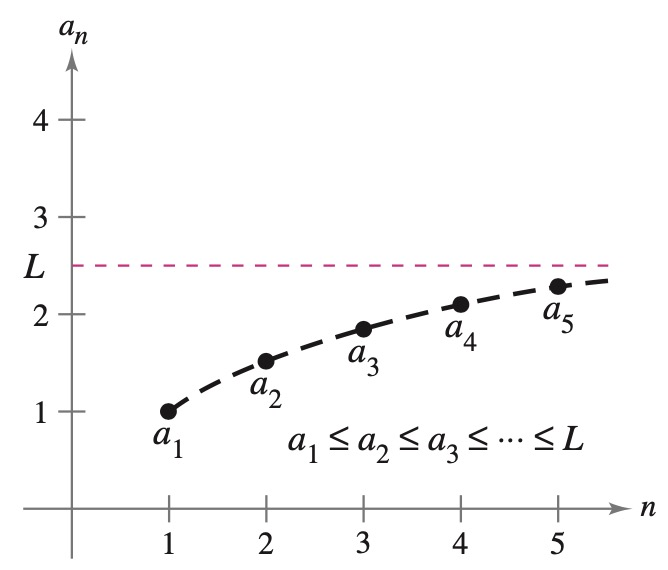
\includegraphics[width=0.55\linewidth]{Example_86.jpg} 
\end{minipage}


\end{mytheorem}

\begin{tcolorbox}[colback=examplebg, colframe=red!75!black, title=\textbf{EXAMPLE 7: Bounded and Monotonic Sequences}, fonttitle=\bfseries, sharp corners]


\begin{enumerate}
    \item The sequence $\{a_n\} = \{1/n\}$ is both bounded and monotonic, and so, by Theorem 9.5, it must converge.

    \item The divergent sequence $\{b_n\} = \{n^2/(n + 1)\}$ is monotonic, but not bounded. (It is bounded below.)

    \item The divergent sequence $\{c_n\} = \{(-1)^n\}$ is bounded, but not monotonic.
\end{enumerate}

\end{tcolorbox}


\subsubsection{Infinite Series}

\begin{Definition}{Infinite Series}{}
    An \textbf{infinite series} is the summation of terms in an infinite sequence $\{a_n\}$, written as:
\[
\sum_{n=1}^\infty a_n = a_1 + a_2 + a_3 + \cdots + a_n + \cdots
\]
The numbers $a_1, a_2, a_3, \dots$ are called the \textbf{terms} of the series.
\end{Definition}

To find the sum of an infinite series, consider the \textbf{sequence of partial sums} listed below:
\[
S_1 = a_1
\]
\[
S_2 = a_1 + a_2
\]
\[
S_3 = a_1 + a_2 + a_3
\]
\[
S_4 = a_1 + a_2 + a_3 + a_4
\]
\[
S_5 = a_1 + a_2 + a_3 + a_4 + a_5
\]
\[
\vdots
\]
\[
S_n = a_1 + a_2 + a_3 + \cdots + a_n
\]

If this sequence of partial sums \textbf{converges}, then the series is said to \textbf{converge} and has the sum indicated by the limiting value of the partial sums.

\begin{Definition}{Convergent and Divergent Series}{}
For the infinite series $\sum_{n=1}^\infty a_n$, the $n$th partial sum is:
\[
S_n = a_1 + a_2 + \cdots + a_n.
\]

If the sequence of partial sums $\{S_n\}$ \textbf{converges} to $S$, then the series $\sum_{n=1}^\infty a_n$ \textbf{converges}. The limit $S$ is called the \textbf{sum of the series}, written as:
\[
S = a_1 + a_2 + \cdots + a_n + \cdots
\]
or:
\[
S = \sum_{n=1}^\infty a_n.
\]

If $\{S_n\}$ \textbf{diverges}, then the series \textbf{diverges}.
\end{Definition}



\begin{tcolorbox}[colback=examplebg, colframe=red!75!black, title=\textbf{EXAMPLE 8: Convergent and Divergent Series}, fonttitle=\bfseries, sharp corners]

\begin{enumerate}
    \item Determine whether the series:
    \[
    \sum_{n=1}^\infty \frac{1}{2^n} = \frac{1}{2} + \frac{1}{4} + \frac{1}{8} + \frac{1}{16} + \cdots
    \]
    converges or diverges.

    \item Find the $n$th partial sum and determine convergence or divergence of the series:
    \[
    \sum_{n=1}^\infty \left( \frac{1}{n} - \frac{1}{n+1} \right).
    \]

    \item Determine whether the series:
    \[
    \sum_{n=1}^\infty 1 = 1 + 1 + 1 + 1 + \cdots
    \]
    converges or diverges.
\end{enumerate}

\tcblower
\textbf{Solution:} 

\begin{enumerate}
    \item The partial sums of the series are:
    \[
    S_1 = \frac{1}{2}, \quad S_2 = \frac{1}{2} + \frac{1}{4} = \frac{3}{4}, \quad S_3 = \frac{1}{2} + \frac{1}{4} + \frac{1}{8} = \frac{7}{8}, \quad \cdots
    \]
    \[
    S_n = \frac{1}{2} + \frac{1}{4} + \frac{1}{8} + \cdots + \frac{1}{2^n} = \frac{2^n - 1}{2^n}.
    \]

    Since:
    \[
    \lim_{n \to \infty} \frac{2^n - 1}{2^n} = 1,
    \]
    the series converges and its sum is $1$.

    \item The $n$th partial sum of the series is:
    \[
    S_n = 1 - \frac{1}{n+1}.
    \]

    As $n \to \infty$, $S_n \to 1$. Thus, the series converges, and its sum is $1$.

    \item The partial sums of the series are:
    \[
    S_n = n.
    \]

    As $n \to \infty$, $S_n \to \infty$. Therefore, the series diverges.
\end{enumerate}
\end{tcolorbox}

\begin{Definition}{Telescoping Series}{}
    A \textbf{telescoping series} is a series where most of the terms cancel out when the series is written as a sum of partial fractions or differences. It is typically of the form:
\[
\sum_{n=1}^\infty (a_n - a_{n+1}),
\]
where many intermediate terms cancel, leaving only the first term $a_1$ and the limiting term (if it exists) as $n \to \infty$.
\end{Definition}

\begin{tcolorbox}[colback=examplebg, colframe=red!75!black, title=\textbf{EXAMPLE 9: Telescoping Series}, fonttitle=\bfseries, sharp corners]

Consider the series:
\[
\sum_{n=1}^\infty \left( \frac{1}{n} - \frac{1}{n+1} \right).
\]

\tcblower
\textbf{Solution:} 
The $n$th partial sum is:
\[
S_n = \left( \frac{1}{1} - \frac{1}{2} \right) + \left( \frac{1}{2} - \frac{1}{3} \right) + \left( \frac{1}{3} - \frac{1}{4} \right) + \cdots + \left( \frac{1}{n} - \frac{1}{n+1} \right).
\]

Most terms cancel, leaving:
\[
S_n = 1 - \frac{1}{n+1}.
\]

Taking the limit as $n \to \infty$:
\[
\lim_{n \to \infty} S_n = 1 - \frac{1}{\infty} = 1.
\]

Thus, the series converges, and its sum is $1$.
\end{tcolorbox}


\newpage
\subsection{Geometric Series}

\begin{Definition}{Geometric Series}{}
    A \textbf{geometric series} is a series of the form:
\[
\sum_{n=0}^\infty ar^n = a + ar + ar^2 + \cdots + ar^n + \cdots,
\]
where $a \neq 0$ and $r \neq 0$ is the \textbf{common ratio}.
\end{Definition}


\begin{mytheorem}{Convergent and Divergent Geometric Series}{}
    
A geometric series with ratio $r$:
\begin{itemize}
    \item \textbf{Diverges} if $\lvert r \rvert \geq 1$.
    \item \textbf{Converges} if $0 < \lvert r \rvert < 1$, and in this case, the sum is given by:
    \[
    \sum_{n=0}^\infty ar^n = \frac{a}{1 - r}, \quad 0 < \lvert r \rvert < 1.
    \]
\end{itemize}
\end{mytheorem}

\textbf{Proof: Convergence and Divergence of a Geometric Series}

It is easy to see that the series diverges when $r = \pm 1$. If $r \neq \pm 1$, then:
\[
S_n = a + ar + ar^2 + \cdots + ar^{n-1}.
\]

Multiplication by $r$ yields:
\[
rS_n = ar + ar^2 + ar^3 + \cdots + ar^n.
\]

Subtracting the second equation from the first produces:
\[
S_n - rS_n = a - ar^n.
\]

Therefore:
\[
S_n(1 - r) = a(1 - r^n),
\]
and the $n$th partial sum is:
\[
S_n = \frac{a}{1 - r}(1 - r^n).
\]

When $0 < \lvert r \rvert < 1$, it follows that $r^n \to 0$ as $n \to \infty$, and you obtain:
\[
\lim_{n \to \infty} S_n = \lim_{n \to \infty} \left[\frac{a}{1 - r}(1 - r^n)\right] = \frac{a}{1 - r} \left[\lim_{n \to \infty}(1 - r^n)\right] = \frac{a}{1 - r}.
\]

This means that the series \textbf{converges} and its sum is $\frac{a}{1 - r}$. 

If $\lvert r \rvert > 1$, the term $r^n$ does not approach $0$ as $n \to \infty$, which means that the series diverges.

\begin{tcolorbox}[colback=examplebg, colframe=red!75!black, title=\textbf{EXAMPLE 1: Convergent and Divergent Geometric Series}, fonttitle=\bfseries, sharp corners]

\begin{enumerate}
    \item Determine if the geometric series     converges or diverges. If it converges, find its sum.
    \[
    \sum_{n=0}^\infty \frac{3}{2^n}
    \]


    \item Determine if the geometric series:
    \[
    \sum_{n=0}^\infty \left(\frac{3}{2}\right)^n
    \]
   
\end{enumerate}

\tcblower
\textbf{Solution:} 
\begin{enumerate}
    \item The series:
    \[
    \sum_{n=0}^\infty \frac{3}{2^n} = \sum_{n=0}^\infty 3\left(\frac{1}{2}\right)^n = 3(1) + 3\left(\frac{1}{2}\right) + 3\left(\frac{1}{2}\right)^2 + \cdots
    \]
    has a ratio $r = \frac{1}{2}$ and $a = 3$. Since $0 < \lvert r \rvert < 1$, the series converges. Its sum is given by:
    \[
    S = \frac{a}{1 - r} = \frac{3}{1 - \frac{1}{2}} = \frac{3}{\frac{1}{2}} = 6.
    \]

    \item The series:
    \[
    \sum_{n=0}^\infty \left(\frac{3}{2}\right)^n = 1 + \frac{3}{2} + \frac{9}{4} + \frac{27}{8} + \cdots
    \]
    has a ratio $r = \frac{3}{2}$. Since $\lvert r \rvert \geq 1$, the series diverges.
\end{enumerate}
\end{tcolorbox}

\begin{tcolorbox}[colback=examplebg, colframe=red!75!black, title=\textbf{EXAMPLE 2:  Geometric Series for a Repeating Decimal}, fonttitle=\bfseries, sharp corners]

Use a geometric series to write $0.\overline{08}$ as the ratio of two integers.

\tcblower
\textbf{Solution:} 
Use a geometric series to write $0.\overline{08}$ as the ratio of two integers.

\textbf{Answer}
For the repeating decimal $0.\overline{08}$, you can write:
\[
0.080808\ldots = \frac{8}{10^2} + \frac{8}{10^4} + \frac{8}{10^6} + \frac{8}{10^8} + \cdots.
\]

This is a geometric series:
\[
\sum_{n=0}^\infty \frac{8}{10^2} \left(\frac{1}{10^2}\right)^n.
\]

For this series, we have $a = \frac{8}{10^2}$ and $r = \frac{1}{10^2}$. Using the formula for the sum of a convergent geometric series:
\[
S = \frac{a}{1 - r},
\]
we get:
\[
0.080808\ldots = \frac{\frac{8}{10^2}}{1 - \frac{1}{10^2}} = \frac{8/100}{1 - 1/100} = \frac{8}{99}.
\]

\textbf{Verification:} Divide $8$ by $99$ using a calculator to confirm it produces $0.\overline{08}$.

\textbf{Additional Note:}

The convergence of a series is not affected by the removal of a finite number of terms from the beginning of the series. For instance, the geometric series:
\[
\sum_{n=4}^\infty \left(\frac{1}{2}\right)^n \quad \text{and} \quad \sum_{n=0}^\infty \left(\frac{1}{2}\right)^n
\]
both converge. 

The sum of the second series is:
\[
S = \frac{a}{1 - r} = \frac{1}{1 - (1/2)} = 2.
\]

You can conclude that the sum of the first series is:
\[
S = 2 - \left[\left(\frac{1}{2}\right)^0 + \left(\frac{1}{2}\right)^1 + \left(\frac{1}{2}\right)^2 + \left(\frac{1}{2}\right)^3\right].
\]

Simplifying:
\[
S = 2 - \frac{15}{8} = \frac{1}{8}.
\]
\end{tcolorbox}

\newpage
\subsection{The nth Term Test
for Divergence}
\begin{mytheorem}{Limit of the $n$th Term of a Convergent Series}{}

    If $\sum_{n=1}^\infty a_n$ converges, then:
\[
\lim_{n \to \infty} a_n = 0.
\]
\end{mytheorem}

\begin{mytheorem}{$n$th-Term Test for Divergence}{}
    If:
\[
\lim_{n \to \infty} a_n \neq 0,
\]
then:
\[
\sum_{n=1}^\infty a_n \quad \text{diverges}.
\]

\end{mytheorem}

\begin{tcolorbox}[colback=examplebg, colframe=red!75!black, title=\textbf{EXAMPLE 1: Using the $n$th-Term Test for Divergence}, fonttitle=\bfseries, sharp corners]
Determine whether the following series diverge using the $n$th-term test:
\begin{enumerate}
    \item $\sum_{n=0}^\infty 2^n$
    \item $\sum_{n=1}^\infty \frac{n!}{2n! + 1}$
    \item $\sum_{n=1}^\infty \frac{1}{n}$
\end{enumerate}


\tcblower
\textbf{Solution:} 
\begin{enumerate}
    \item For the series $\sum_{n=0}^\infty 2^n$, we have:
    \[
    \lim_{n \to \infty} 2^n = \infty.
    \]
    Since the limit of the $n$th term is not $0$, the series diverges.

    \item For the series $\sum_{n=1}^\infty \frac{n!}{2n! + 1}$, we have:
    \[
    \lim_{n \to \infty} \frac{n!}{2n! + 1} = \frac{1}{2}.
    \]
    Since the limit of the $n$th term is not $0$, the series diverges.

    \item For the series $\sum_{n=1}^\infty \frac{1}{n}$, we have:
    \[
    \lim_{n \to \infty} \frac{1}{n} = 0.
    \]
    Since the limit of the $n$th term is $0$, the $n$th-term test does not determine whether the series converges or diverges. 
\end{enumerate}
\end{tcolorbox}


\subsection{Integral Test for
Convergence}
\begin{mytheorem}{The Integral Test}{}

If $f$ is positive, continuous, and decreasing for $x \geq 1$ and $a_n = f(n)$, then:
\[
\sum_{n=1}^\infty a_n \quad \text{and} \quad \int_1^\infty f(x) \, dx
\]
either both converge or both diverge.
    
\end{mytheorem}

\begin{tcolorbox}[colback=examplebg, colframe=red!75!black, title=\textbf{EXAMPLE 1: Using the Integral Test}, fonttitle=\bfseries, sharp corners]
Apply the Integral Test to the series:
\[
\sum_{n=1}^\infty \frac{n}{n^2 + 1}.
\]


\tcblower
\textbf{Solution:} 
The function $f(x) = \frac{x}{x^2 + 1}$ is positive and continuous for $x \geq 1$. To determine whether $f$ is decreasing, find its derivative:
\[
f'(x) = \frac{(x^2 + 1)(1) - x(2x)}{(x^2 + 1)^2} = \frac{-x^2 + 1}{(x^2 + 1)^2}.
\]

Since $f'(x) < 0$ for $x > 1$, it follows that $f$ satisfies the conditions for the Integral Test. Integrating, we have:
\[
\int_1^\infty \frac{x}{x^2 + 1} \, dx = \frac{1}{2} \int_1^\infty \frac{2x}{x^2 + 1} \, dx.
\]

Let $u = x^2 + 1$, so $du = 2x \, dx$:
\[
\int_1^\infty \frac{x}{x^2 + 1} \, dx = \frac{1}{2} \int_1^\infty \frac{du}{u}.
\]

Evaluate the integral:
\[
\frac{1}{2} \int_1^\infty \frac{du}{u} = \frac{1}{2} \lim_{b \to \infty} \int_1^b \frac{du}{u} = \frac{1}{2} \lim_{b \to \infty} [\ln(u)]_1^b.
\]

Substitute $u = x^2 + 1$ back:
\[
= \frac{1}{2} \lim_{b \to \infty} [\ln(b^2 + 1) - \ln(2)] = \infty.
\]

Since the integral diverges, the series also diverges.
\end{tcolorbox}



\begin{tcolorbox}[colback=examplebg, colframe=red!75!black, title=\textbf{EXAMPLE 2: Using the Integral Test}, fonttitle=\bfseries, sharp corners]

Apply the Integral Test to the series:
\[
\sum_{n=1}^\infty \frac{1}{n^2 + 1}.
\]
\begin{minipage}{\linewidth}
    \centering
    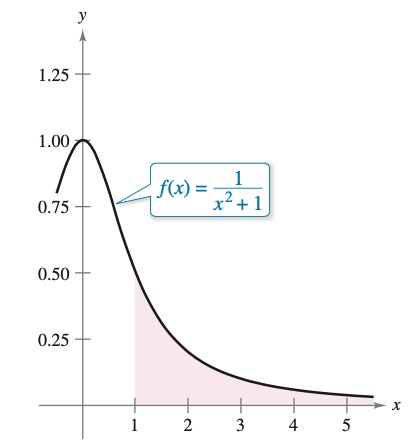
\includegraphics[width=0.40\linewidth]{Example_87.jpg} 
\end{minipage}
\tcblower
\textbf{Solution:} 
The function $f(x) = \frac{1}{x^2 + 1}$ satisfies the conditions for the Integral Test. Integrate:
\[
\int_1^\infty \frac{1}{x^2 + 1} \, dx = \lim_{b \to \infty} \int_1^b \frac{1}{x^2 + 1} \, dx.
\]

The antiderivative of $\frac{1}{x^2 + 1}$ is $\arctan(x)$:
\[
\int_1^\infty \frac{1}{x^2 + 1} \, dx = \lim_{b \to \infty} [\arctan(x)]_1^b.
\]

Evaluate:
\[
\lim_{b \to \infty} [\arctan(b) - \arctan(1)] = \frac{\pi}{2} - \frac{\pi}{4} = \frac{\pi}{4}.
\]

Since the integral converges, the series also converges.


\end{tcolorbox}
\newpage
\subsection{Harmonic Series
and p-Series}
\begin{Definition}{P Series}{}
    A series of the form:
\[
\sum_{n=1}^\infty \frac{1}{n^p} = \frac{1}{1^p} + \frac{1}{2^p} + \frac{1}{3^p} + \cdots
\]
is called a \textbf{p-series}, where $p$ is a positive constant.
\end{Definition}


\begin{Definition}{Harmonic Series}{}
For $p = 1$, the series:
\[
\sum_{n=1}^\infty \frac{1}{n} = 1 + \frac{1}{2} + \frac{1}{3} + \cdots
\]
is the \textbf{harmonic series}.
\end{Definition}

\begin{mytheorem}{ Convergence of $p$-Series}{}
    The $p$-series:
\[
\sum_{n=1}^\infty \frac{1}{n^p} = \frac{1}{1^p} + \frac{1}{2^p} + \frac{1}{3^p} + \frac{1}{4^p} + \cdots
\]
\begin{itemize}
    \item \textbf{Converges} for $p > 1$.
    \item \textbf{Diverges} for $0 < p \leq 1$.
\end{itemize}
\end{mytheorem}

\begin{tcolorbox}[colback=examplebg, colframe=red!75!black, title=\textbf{EXAMPLE 1: Convergent and Divergent $p$-Series}, fonttitle=\bfseries, sharp corners]

Discuss the convergence or divergence of:
\begin{enumerate}
    \item The harmonic series.
    \item The $p$-series with $p = 2$.
\end{enumerate}

\tcblower
\textbf{Solution:} 
\begin{enumerate}
    \item From Theorem, it follows that the harmonic series:
    \[
    \sum_{n=1}^\infty \frac{1}{n} = 1 + \frac{1}{2} + \frac{1}{3} + \cdots
    \]
    diverges because $p = 1$.

    \item From Theorem, it follows that the $p$-series:
    \[
    \sum_{n=1}^\infty \frac{1}{n^2} = \frac{1}{1^2} + \frac{1}{2^2} + \frac{1}{3^2} + \cdots
    \]
    converges because $p = 2 > 1$.
\end{enumerate}
\end{tcolorbox}

\newpage
\subsection{Comparison Tests
for Convergence}

\subsubsection{Comparison Tests
for Convergence}
\begin{mytheorem}{Direct Comparison Test}{}
Let $0 < a_n \leq b_n$ for all $n$.

\begin{enumerate}
    \item If $\sum_{n=1}^\infty b_n$ converges, then $\sum_{n=1}^\infty a_n$ converges.
    \item If $\sum_{n=1}^\infty a_n$ diverges, then $\sum_{n=1}^\infty b_n$ diverges.
\end{enumerate}
\end{mytheorem}


\begin{tcolorbox}[colback=examplebg, colframe=red!75!black, title=\textbf{EXAMPLE 1: Direct Comparison Test}, fonttitle=\bfseries, sharp corners]
Determine whether the series 
\[
\sum_{n=1}^\infty \frac{5}{2n^2 + 4n + 3}
\]
converges or diverges.



\tcblower
\textbf{Solution:} 
For large $n$, the dominant term in the denominator is $2n^2$, so we compare the given series with the series $\sum \frac{5}{2n^2}$. Observe that
\[
\frac{5}{2n^2 + 4n + 3} < \frac{5}{2n^2},
\]

is convergent because it’s a constant times a $p$-series with $p = 2 > 1$. Therefore,
\[
\sum_{n=1}^\infty \frac{5}{2n^2 + 4n + 3}
\]
is convergent by using the Direct Comparison Test.
\end{tcolorbox}



\begin{tcolorbox}[colback=examplebg, colframe=red!75!black, title=\textbf{EXAMPLE 2: Direct Comparison Test}, fonttitle=\bfseries, sharp corners]

Test the series 
\[
\sum_{k=1}^\infty \frac{\ln k}{k}
\]
for convergence or divergence.


\tcblower
\textbf{Solution:} 
By comparing it with the harmonic series. Observe that
\[
\frac{\ln k}{k} > \frac{1}{k}, \quad k \geq 3.
\]

We know that $\sum \frac{1}{k}$ is divergent (a $p$-series with $p = 1$). Thus the given series is divergent by the Direct Comparison Test.
\end{tcolorbox}


\subsubsection{The Limit Comparison Test}

\begin{mytheorem}{The Limit Comparison Test}{}
    If $a_n > 0$, $b_n > 0$, and
\[
\lim_{n \to \infty} \frac{a_n}{b_n} = L,
\]
where $L$ is finite and positive, then
\[
\sum_{n=1}^\infty a_n \quad \text{and} \quad \sum_{n=1}^\infty b_n
\]
either both converge or both diverge.
\end{mytheorem}

\begin{tcolorbox}[colback=examplebg, colframe=red!75!black, title=\textbf{EXAMPLE 3: The Limit Comparison Test}, fonttitle=\bfseries, sharp corners]

Test the series
\[
\sum_{n=1}^\infty \frac{1}{2^n - 1}
\]
for convergence or divergence.

\tcblower
\textbf{Solution:} 
We use the Limit Comparison Test with
\[
a_n = \frac{1}{2^n - 1}, \quad b_n = \frac{1}{2^n},
\]
and obtain
\[
\lim_{n \to \infty} \frac{a_n}{b_n} = \lim_{n \to \infty} \frac{\frac{1}{2^n - 1}}{\frac{1}{2^n}} = \lim_{n \to \infty} \frac{2^n}{2^n - 1} = \lim_{n \to \infty} \frac{1}{1 - \frac{1}{2^n}} = 1 > 0.
\]
Since $\sum_{n=1}^\infty b_n = \sum_{n=1}^\infty \frac{1}{2^n}$ converges (geometric series), the given series $\sum_{n=1}^\infty a_n$ converges by the Limit Comparison Test.
\end{tcolorbox}

\begin{tcolorbox}[colback=examplebg, colframe=red!75!black, title=\textbf{EXAMPLE 4: The Limit Comparison Test}, fonttitle=\bfseries, sharp corners]

Determine whether the series
\[
\sum_{n=1}^\infty \frac{2n^2 + 3n}{\sqrt{5 + n^5}}
\]
converges or diverges.

\tcblower
\textbf{Solution:} 
The dominant part of the numerator is $2n^2$, and the dominant part of the denominator is $\sqrt{n^5} = n^{5/2}$. This suggests taking
\[
a_n = \frac{2n^2 + 3n}{\sqrt{5 + n^5}}, \quad b_n = \frac{2n^2}{n^{5/2}} = \frac{2}{n^{1/2}}.
\]

We compute
\[
\lim_{n \to \infty} \frac{a_n}{b_n} = \lim_{n \to \infty} \frac{\frac{2n^2 + 3n}{\sqrt{5 + n^5}}}{\frac{2}{n^{1/2}}} = \lim_{n \to \infty} \frac{2n^2 + 3n}{\sqrt{5 + n^5}} \cdot \frac{n^{1/2}}{2}.
\]
Simplify:
\[
\lim_{n \to \infty} \frac{a_n}{b_n} = \lim_{n \to \infty} \frac{2n^{5/2} + 3n^{3/2}}{2\sqrt{5 + n^5}} = \lim_{n \to \infty} \frac{2n^{5/2} + 3n^{3/2}}{2n^{5/2}}.
\]
Divide through by $n^{5/2}$:
\[
\lim_{n \to \infty} \frac{a_n}{b_n} = \frac{2 + \frac{3}{n}}{2 + \frac{\sqrt{5}}{n^5}} = \frac{2 + 0}{2 + 0} = 1.
\]

Since $\sum b_n = \sum \frac{2}{n^{1/2}} = 2\sum \frac{1}{n^{1/2}}$ is divergent (a $p$-series with $p = 1/2 < 1$), the given series diverges by the Limit Comparison Test
\end{tcolorbox}

\newpage

\subsection{Alternating Series}

\begin{Definition}{Alternating Series}{}
The series
\[
\sum_{n=0}^\infty \left( -\frac{1}{2} \right)^n = \sum_{n=0}^\infty (-1)^n \frac{1}{2^n}
\]
can be expanded as
\[
= 1 - \frac{1}{2} + \frac{1}{4} - \frac{1}{8} + \frac{1}{16} - \cdots.
\]

This is an \textbf{alternating geometric series} with $r = -\frac{1}{2}$. Alternating series occur in two ways:
\begin{itemize}
    \item Either the odd terms are negative.
    \item Or the even terms are negative.
\end{itemize}

    
\end{Definition}

\begin{mytheorem}{ Alternating Series Test}{}

Let $a_n > 0$. The alternating series
\[
\sum_{n=1}^\infty (-1)^n a_n \quad \text{and} \quad \sum_{n=1}^\infty (-1)^{n+1} a_n
\]
converge when the two conditions listed below are met:
\begin{enumerate}
    \item $\lim_{n \to \infty} a_n = 0$,
    \item $a_{n+1} \leq a_n$, for all $n$.
\end{enumerate}
\end{mytheorem}
\begin{tcolorbox}[colback=examplebg, colframe=red!75!black, title=\textbf{EXAMPLE 1: Using the Alternating Series Test}, fonttitle=\bfseries, sharp corners]

Determine the convergence or divergence of
\[
\sum_{n=1}^\infty (-1)^{n+1} \frac{1}{n}.
\]

\tcblower
\textbf{Solution:} 
Note that
\[
\lim_{n \to \infty} a_n = \lim_{n \to \infty} \frac{1}{n} = 0.
\]
So, the first condition of Theorem is satisfied. Also, the second condition of Theorem is satisfied because
\[
a_{n+1} = \frac{1}{n+1} \leq \frac{1}{n} = a_n,
\]
for all $n$. Thus, applying the Alternating Series Test, we conclude that the series converges.
\end{tcolorbox}

\begin{tcolorbox}[colback=examplebg, colframe=red!75!black, title=\textbf{EXAMPLE 2: Using the Alternating Series Test}, fonttitle=\bfseries, sharp corners]

Determine the convergence or divergence of
\[
\sum_{n=1}^\infty \frac{n}{(-2)^{n-1}}.
\]

\tcblower
\textbf{Solution:} 
To apply the Alternating Series Test, note that, for $n \geq 1$,
\[
\frac{1}{2} \leq \frac{n}{n+1}.
\]
Simplify:
\[
\frac{2n - 1}{2n} \leq \frac{n}{n+1}.
\]
By L’Hôpital's Rule:
\[
\lim_{n\to\infty} \frac{x}{x^n} = 0.
\]
Therefore, by the Alternating Series Test, the series converges.
\end{tcolorbox}

\begin{tcolorbox}[colback=examplebg, colframe=red!75!black, title=\textbf{EXAMPLE 3: Using the Alternating Series Test}, fonttitle=\bfseries, sharp corners]

Determine the series
\[
\sum_{n=1}^\infty (-1)^n \frac{3n}{4n - 1}
\]
is convergent or divergent

\tcblower
\textbf{Solution:} 
The series
\[
\sum_{n=1}^\infty (-1)^n \frac{3n}{4n - 1}
\]
is alternating, but
\[
\lim_{n \to \infty} b_n = \lim_{n \to \infty} \frac{3n}{4n - 1} = \lim_{n \to \infty} \frac{3}{4 - \frac{1}{n}} = \frac{3}{4}.
\]

Since $\lim_{n \to \infty} b_n \neq 0$, condition (i) is not satisfied. Thus, the Alternating Series Test does not apply.

Instead, we examine the limit of the $n$th term of the series:
\[
\lim_{n \to \infty} a_n = \lim_{n \to \infty} (-1)^n \frac{3n}{4n - 1}.
\]

This limit does not exist due to the oscillating $(-1)^n$ factor. Therefore, the series diverges by the \textbf{Test for Divergence}.
\end{tcolorbox}


\subsection{Ratio Test for
Convergence}

\begin{mytheorem}{The Ratio Test}{}
    \begin{enumerate}
    \item[(i)] If 
    \[
    \lim_{n \to \infty} \left| \frac{a_{n+1}}{a_n} \right| = L < 1,
    \]
    then the series $\sum_{n=1}^\infty a_n$ is absolutely convergent (and therefore convergent).

    \item[(ii)] If 
    \[
    \lim_{n \to \infty} \left| \frac{a_{n+1}}{a_n} \right| = L > 1 \quad \text{or} \quad \lim_{n \to \infty} \left| \frac{a_{n+1}}{a_n} \right| = \infty,
    \]
    then the series $\sum_{n=1}^\infty a_n$ is divergent.

    \item[(iii)] If 
    \[
    \lim_{n \to \infty} \left| \frac{a_{n+1}}{a_n} \right| = 1,
    \]
    the Ratio Test is inconclusive; that is, no conclusion can be drawn about the convergence or divergence of $\sum_{n=1}^\infty a_n$.
\end{enumerate}
\end{mytheorem}

For the \textbf{absolutely convergent}, we will talk about it in the next chapter

\begin{tcolorbox}[colback=examplebg, colframe=red!75!black, title=\textbf{EXAMPLE 1: Using the Ratio Test}, fonttitle=\bfseries, sharp corners]
Test the series 
\[
\sum_{n=1}^\infty (-1)^n \frac{n^3}{3^n}
\]
for convergence.


\tcblower
\textbf{Solution:} 
We use the Ratio Test with $a_n = (-1)^n \frac{n^3}{3^n}$:
\[
\left| \frac{a_{n+1}}{a_n} \right| = \left| \frac{(-1)^{n+1}(n+1)^3 / 3^{n+1}}{(-1)^n n^3 / 3^n} \right| = \frac{(n+1)^3}{3^{n+1}} \cdot \frac{3^n}{n^3}.
\]
Simplify:
\[
\left| \frac{a_{n+1}}{a_n} \right| = \frac{(n+1)^3}{3n^3}.
\]
Factor and take the limit:
\[
= \frac{1}{3} \left( 1 + \frac{1}{n} \right)^3 \to \frac{1}{3} (1)^3 = \frac{1}{3}.
\]
Since $\frac{1}{3} < 1$, the given series is convergent by the Ratio Test.
\end{tcolorbox}



\begin{tcolorbox}[colback=examplebg, colframe=red!75!black, title=\textbf{EXAMPLE 2: Using the Ratio Test}, fonttitle=\bfseries, sharp corners]
Test the convergence of the series 
\[
\sum_{n=1}^\infty \frac{n^n}{n!}.
\]


\tcblower
\textbf{Solution:} 
Since the terms $a_n = \frac{n^n}{n!}$ are positive, we don’t need the absolute value signs. Compute:
\[
\frac{a_{n+1}}{a_n} = \frac{(n+1)^{n+1}}{(n+1)!} \cdot \frac{n!}{n^n}.
\]
Simplify:
\[
= \frac{(n+1)(n+1)^n}{(n+1)n^n} = \left( 1 + \frac{1}{n} \right)^n \to e \quad \text{as } n \to \infty.
\]
Since $e > 1$, the given series diverges by the Ratio Test.

\end{tcolorbox}







\begin{tcolorbox}[colback=examplebg, colframe=red!75!black, title=\textbf{EXAMPLE 3: A Failure of the Ratio Test}, fonttitle=\bfseries, sharp corners]

Determine the convergence or divergence of
\[
\sum_{n=1}^\infty (-1)^n \frac{\sqrt{n}}{n+1}.
\]

\tcblower
\textbf{Solution:} 
The limit of $\left| \frac{a_{n+1}}{a_n} \right|$ is computed as follows:
\[
\lim_{n \to \infty} \left| \frac{a_{n+1}}{a_n} \right| = \lim_{n \to \infty} \left( \frac{\sqrt{n+1}}{n+2} \cdot \frac{n+1}{\sqrt{n}} \right).
\]
Simplify:
\[
= \lim_{n \to \infty} \sqrt{\frac{n+1}{n}} \cdot \frac{n+1}{n+2}.
\]
Factor:
\[
= \lim_{n \to \infty} \sqrt{\frac{n+1}{n}} \cdot \left( 1 - \frac{1}{n+2} \right) = \sqrt{1}(1) = 1.
\]
Since the limit equals $1$, the Ratio Test is inconclusive.
\end{tcolorbox}

\newpage


\subsection{Absolute
or Conditional
Convergence}

Consider the series
\[
\sum_{n=1}^\infty \frac{\sin n}{n^3}.
\]

This series has both positive and negative terms, but it is not an alternating series. To investigate its convergence, we examine the series of absolute values:
\[
\sum_{n=1}^\infty \left| \frac{\sin n}{n^3} \right|.
\]

Since $|\sin n| \leq 1$ for all $n$, we have
\[
\left| \frac{\sin n}{n^3} \right| \leq \frac{1}{n^3}.
\]

The series $\sum_{n=1}^\infty \frac{1}{n^3}$ is a $p$-series with $p = 3 > 1$, so it converges. By the Direct Comparison Test, the series
\[
\sum_{n=1}^\infty \left| \frac{\sin n}{n^3} \right|
\]
also converges.

The next theorem will tell you that the original series is also convergent.

\begin{Definition}{Absolute and Conditional Convergence}{}

\begin{enumerate}
    \item The series $\sum a_n$ is \textbf{absolutely convergent} when $\sum |a_n|$ converges.
    \item The series $\sum a_n$ is \textbf{conditionally convergent} when $\sum a_n$ converges but $\sum |a_n|$ diverges.
\end{enumerate}

    
\end{Definition}

\begin{mytheorem}{Absolute Convergence}{}   
If the series $\sum |a_n|$ converges, then the series $\sum a_n$ also converges.

\end{mytheorem}

\begin{tcolorbox}[colback=examplebg, colframe=red!75!black, title=\textbf{EXAMPLE 1: Absolute or Conditional Convergence}, fonttitle=\bfseries, sharp corners]
 Determine Whether the Series is Absolutely Convergent, Conditionally Convergent, or Divergent
\begin{enumerate}
    \item[(a)] \[
    \sum_{n=1}^\infty \frac{(-1)^n}{n^3}
    \]
    \item[(b)] \[
    \sum_{n=1}^\infty \frac{(-1)^n}{\sqrt[3]{n}}
    \]
    \item[(c)] \[
    \sum_{n=1}^\infty (-1)^n \frac{n}{2n + 1}
    \]
\end{enumerate}

\tcblower
\textbf{Solution:} 
\begin{enumerate}
    \item[(a)] Because the series
    \[
    \sum_{n=1}^\infty \left| \frac{(-1)^n}{n^3} \right| = \sum_{n=1}^\infty \frac{1}{n^3}
    \]
    converges (a $p$-series with $p = 3 > 1$), the given series is \textbf{absolutely convergent}.

    \item[(b)] We first test for absolute convergence. The series
    \[
    \sum_{n=1}^\infty \left| \frac{(-1)^n}{\sqrt[3]{n}} \right| = \sum_{n=1}^\infty \frac{1}{\sqrt[3]{n}}
    \]
    diverges (a $p$-series with $p = \frac{1}{3} < 1$), so the given series is not absolutely convergent.

    The given series converges by the Alternating Series Test (since $b_{n+1} \leq b_n$ and $\lim_{n \to \infty} b_n = 0$). Since the series converges but is not absolutely convergent, it is \textbf{conditionally convergent}.

    \item[(c)] This series is alternating, but
    \[
    \lim_{n \to \infty} a_n = \lim_{n \to \infty} (-1)^n \frac{n}{2n + 1}
    \]
    does not exist. Therefore, the series diverges by the \textbf{Test for Divergence}.
\end{enumerate}
\end{tcolorbox}

\begin{tcolorbox}[colback=examplebg, colframe=red!75!black, title=\textbf{EXAMPLE 2: bsolute or Conditional Convergence}, fonttitle=\bfseries, sharp corners]
Determine whether each of the series is convergent or divergent. Classify any convergent series as absolutely or conditionally convergent.
\begin{enumerate}
    \item[(a)] \[
    \sum_{n=0}^\infty \frac{(-1)^n n!}{2^n} = \frac{0!}{2^0} - \frac{1!}{2^1} + \frac{2!}{2^2} - \frac{3!}{2^3} + \cdots
    \]
    \item[(b)] \[
    \sum_{n=1}^\infty \frac{(-1)^n}{\sqrt{n}} = -\frac{1}{\sqrt{1}} + \frac{1}{\sqrt{2}} - \frac{1}{\sqrt{3}} + \frac{1}{\sqrt{4}} - \cdots
    \]
\end{enumerate}


\tcblower
\textbf{Solution:} 
\begin{enumerate}
    \item[(a)] This is an alternating series, but the Alternating Series Test does not apply because the limit of the $n$th term is not zero:
    \[
    \lim_{n \to \infty} \frac{(-1)^n n!}{2^n} \neq 0.
    \]
    By the $n$th-Term Test for Divergence, this series diverges.

    \item[(b)] This series can be shown to be convergent by the Alternating Series Test. Moreover, because the $p$-series
    \[
    \sum_{n=1}^\infty \left| \frac{(-1)^n}{\sqrt{n}} \right| = \sum_{n=1}^\infty \frac{1}{\sqrt{n}}
    \]
    diverges (since $p = \frac{1}{2} < 1$), the given series is \textbf{conditionally convergent}.
\end{enumerate}
\end{tcolorbox}

\newpage

\subsection{Alternating Series
Error Bound}

For a convergent alternating series, the partial sum $S_N$ can be a useful approximation for the sum $S$ of the series. The error involved in using $S \approx S_N$ is the remainder
\[
R_N = S - S_N.
\]
\begin{mytheorem}{Alternating Series Remainder}{}
    If a convergent alternating series satisfies the condition $a_{n+1} \leq a_n$, then the absolute value of the remainder $R_N$ involved in approximating the sum $S$ by $S_N$ is less than (or equal to) the first neglected term. That is,
\[
|S - S_N| = |R_N| \leq a_{N+1}.
\]

\end{mytheorem}



\begin{tcolorbox}[colback=examplebg, colframe=red!75!black, title=\textbf{EXAMPLE 1: Finding the Number of Terms}, fonttitle=\bfseries, sharp corners]

Determine the number of terms required to approximate the sum of the series with an error of less than $0.001$:
\[
\sum_{n=1}^\infty \frac{(-1)^{n+1}}{n^4}.
\]

\tcblower
\textbf{Solution:} 
\[
|R_N| \leq a_{N+1} = \frac{1}{(N+1)^4}.
\]

For an error of less than $0.001$, $N$ must satisfy the inequality
\[
\frac{1}{(N+1)^4} < 0.001 \quad \Rightarrow \quad (N+1)^4 > 1000 \quad \Rightarrow \quad N+1 > \sqrt[4]{1000} \quad \Rightarrow \quad N > \sqrt[4]{1000} - 1 \approx 4.6.
\]

So, you will need at least 5 terms. Using 5 terms, the sum is
\[
S \approx S_5 \approx 0.94754,
\]
which has an error of less than $0.001$.
\end{tcolorbox}

\begin{tcolorbox}[colback=examplebg, colframe=red!75!black, title=\textbf{EXAMPLE 2: Find the Sum of the Series}, fonttitle=\bfseries, sharp corners]

Find the Sum of the Series Correct to Three Decimal Places
\[
\sum_{n=0}^\infty \frac{(-1)^n}{n!}
\]

\tcblower
\textbf{Solution:} 
We first observe that the series is convergent by the Alternating Series Test because
\begin{enumerate}
    \item[(i)] \[
    b_{n+1} = \frac{1}{(n+1)!} = \frac{1}{n!(n+1)} < \frac{1}{n!} = b_n
    \]
    \item[(ii)] \[
    0 < \frac{1}{n!} < \frac{1}{n} \to 0 \quad \text{as } n \to \infty, \quad \text{so } b_n = \frac{1}{n!} \to 0 \text{ as } n \to \infty.
    \]
\end{enumerate}

To get a feel for how many terms we need to use in our approximation, let’s write out the first few terms of the series:
\[
s = \frac{1}{0!} - \frac{1}{1!} + \frac{1}{2!} - \frac{1}{3!} + \frac{1}{4!} - \frac{1}{5!} + \frac{1}{6!} - \frac{1}{7!} + \cdots
\]
\[
= 1 - 1 + \frac{1}{2} - \frac{1}{6} + \frac{1}{24} - \frac{1}{120} + \frac{1}{720} - \frac{1}{5040} + \cdots
\]

Notice that
\[
b_7 = \frac{1}{5040} < \frac{1}{5000} = 0.0002,
\]
and
\[
s_6 = 1 - 1 + \frac{1}{2} - \frac{1}{6} + \frac{1}{24} - \frac{1}{120} + \frac{1}{720} \approx 0.368056.
\]

By the Alternating Series Estimation Theorem, we know that
\[
|s - s_6| \leq b_7 < 0.0002.
\]

This error of less than 0.0002 does not affect the third decimal place, so we have
\[
s \approx 0.368 \quad \text{correct to three decimal places.}
\]
\end{tcolorbox}


\begin{tcolorbox}[colback=examplebg, colframe=red!75!black, title=\textbf{EXAMPLE 3: Approximating the Sum of an Alternating Series}, fonttitle=\bfseries, sharp corners]
Approximating the Sum of an Alternating Series by its first six terms
\[
\sum_{n=1}^\infty (-1)^{n+1} \left( \frac{1}{n!} \right) = \frac{1}{1!} - \frac{1}{2!} + \frac{1}{3!} - \frac{1}{4!} + \frac{1}{5!} - \frac{1}{6!} + \cdots
\]


\tcblower
\textbf{Solution:} 
The series converges by the Alternating Series Test because
\[
\frac{1}{(n+1)!} \leq \frac{1}{n!} \quad \text{and} \quad \lim_{n \to \infty} \frac{1}{n!} = 0.
\]

The sum of the first six terms is
\[
S_6 = 1 - \frac{1}{2} + \frac{1}{6} - \frac{1}{24} + \frac{1}{120} - \frac{1}{720} = \frac{91}{144} \approx 0.63194.
\]

By the Alternating Series Remainder Theorem, you have
\[
|S - S_6| = |R_6| \leq a_7 = \frac{1}{5040} \approx 0.0002.
\]

So, the sum $S$ lies between
\[
0.63194 - 0.0002 \quad \text{and} \quad 0.63194 + 0.0002,
\]
and you have
\[
0.63174 \leq S \leq 0.63214.
\]
\end{tcolorbox}


\newpage
\subsection{Taylor Polynomial
Approximations of Functions}

\subsubsection{Polynomial Approximations of Elementary Functions}
Polynomial approximations of elementary functions refer to the representation of functions (such as exponential functions, logarithms etc.) as polynomials that approximate the original functions within a certain range. 

\begin{Definition}{Polynomial Approximations of Elementary Functions}{}
    A polynomial approximation of a function $f(x)$ is a polynomial $P_n(x)$ of degree $n$ such that:
\[
P_n(x) = f(a) + f'(a)(x-a) + \frac{f''(a)}{2!}(x-a)^2 + \cdots + \frac{f^{(n)}(a)}{n!}(x-a)^n,
\]
where $a$ is a point around which the function is approximated.

\end{Definition}

\begin{tcolorbox}[colback=examplebg, colframe=red!75!black, title=\textbf{EXAMPLE 1: First-Degree Polynomial Approximation of $f(x) = e^x$}, fonttitle=\bfseries, sharp corners]

For the function $f(x) = e^x$, find a first-degree polynomial function $P_1(x) = a_0 + a_1x$ whose value and slope agree with the value and slope of $f$ at $x = 0$.


\tcblower
\textbf{Solution:} 
Because $f(x) = e^x$ and $f'(x) = e^x$, the value and the slope of $f$ at $x = 0$ are
\[
f(0) = e^0 = 1 \quad \text{(Value of $f$ at $x=0$)}
\]
and
\[
f'(0) = e^0 = 1 \quad \text{(Slope of $f$ at $x=0$)}.
\]

Because $P_1(x) = a_0 + a_1x$, you can use the condition that $P_1(0) = f(0)$ to conclude that $a_0 = 1$. Moreover, because $P_1'(x) = a_1$, you can use the condition that $P_1'(0) = f'(0)$ to conclude that $a_1 = 1$. Therefore,
\[
P_1(x) = 1 + x.
\]

The figure below shows the graphs of $P_1(x) = 1 + x$ and $f(x) = e^x$:


$P_1$ is the first-degree polynomial approximation of $f(x) = e^x$.

\begin{minipage}{\linewidth}
    \centering
    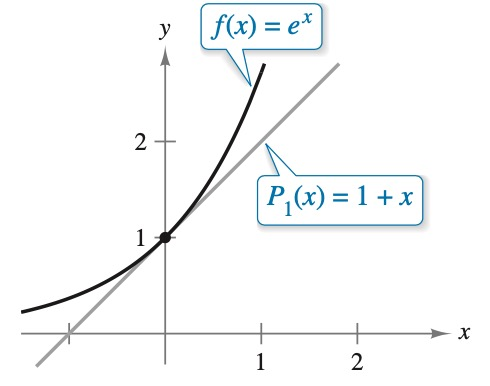
\includegraphics[width=0.30\linewidth]{Example_88.jpg} 
\end{minipage}

\end{tcolorbox}


\subsubsection{Taylor and Maclaurin Polynomials}
\begin{Definition}{$n$th Taylor Polynomial and $n$th Maclaurin Polynomial}{}
If $f$ has $n$ derivatives at $c$, then the polynomial
\[
P_n(x) = f(c) + f'(c)(x-c) + \frac{f''(c)}{2!}(x-c)^2 + \cdots + \frac{f^{(n)}(c)}{n!}(x-c)^n
\]
is called the \textbf{$n$th Taylor polynomial} for $f$ at $c$. 

If $c = 0$, then
\[
P_n(x) = f(0) + f'(0)x + \frac{f''(0)}{2!}x^2 + \frac{f^{(3)}(0)}{3!}x^3 + \cdots + \frac{f^{(n)}(0)}{n!}x^n
\]
is also called the \textbf{$n$th Maclaurin polynomial} for $f$.
\end{Definition}


\begin{tcolorbox}[colback=examplebg, colframe=red!75!black, title=\textbf{EXAMPLE 2: A Maclaurin Polynomial for $f(x) = e^x$}, fonttitle=\bfseries, sharp corners]

Find the $n$th Maclaurin polynomial for 
\[
f(x) = e^x.
\]

\tcblower
\textbf{Solution:} 
From the discussion on the preceding page, the $n$th Maclaurin polynomial for $f(x) = e^x$ is
\[
P_n(x) = 1 + x + \frac{1}{2!}x^2 + \frac{1}{3!}x^3 + \cdots + \frac{1}{n!}x^n.
\]
\end{tcolorbox}


\begin{tcolorbox}[colback=examplebg, colframe=red!75!black, title=\textbf{EXAMPLE 3: Finding Taylor Polynomials for $\ln x$}, fonttitle=\bfseries, sharp corners]
Find the Taylor polynomials $P_0$, $P_1$, $P_2$, $P_3$, and $P_4$ for 
\[
f(x) = \ln x,
\]
centered at $c = 1$


\tcblower
\textbf{Solution:} 
Expanding about $c = 1$ yields the following:
\[
\begin{aligned}
f(x) &= \ln x, & f(1) &= \ln 1 = 0, \\
f'(x) &= \frac{1}{x}, & f'(1) &= \frac{1}{1} = 1, \\
f''(x) &= -\frac{1}{x^2}, & f''(1) &= -\frac{1}{1^2} = -1, \\
f'''(x) &= \frac{2!}{x^3}, & f'''(1) &= \frac{2!}{1^3} = 2, \\
f^{(4)}(x) &= -\frac{3!}{x^4}, & f^{(4)}(1) &= -\frac{3!}{1^4} = -6.
\end{aligned}
\]

Therefore, the Taylor polynomials are as follows:
\[
\begin{aligned}
P_0(x) &= f(1) = 0, \\
P_1(x) &= f(1) + f'(1)(x-1) = (x-1), \\
P_2(x) &= f(1) + f'(1)(x-1) + \frac{f''(1)}{2!}(x-1)^2 = (x-1) - \frac{1}{2}(x-1)^2, \\
P_3(x) &=  (x-1) - \frac{1}{2}(x-1)^2 + \frac{1}{3}(x-1)^3, \\
P_4(x) &= f(1) + f'(1)(x-1) + \frac{f''(1)}{2!}(x-1)^2 + \frac{f'''(1)}{3!}(x-1)^3 + \frac{f^{(4)}(1)}{4!}(x-1)^4 \\
&= (x-1) - \frac{1}{2}(x-1)^2 + \frac{1}{3}(x-1)^3 - \frac{1}{4}(x-1)^4.
\end{aligned}
\]
\end{tcolorbox}


\begin{tcolorbox}[colback=examplebg, colframe=red!75!black, title=\textbf{EXAMPLE 4: Finding Maclaurin Polynomials for $\cos x$}, fonttitle=\bfseries, sharp corners]
Find the Maclaurin polynomials $P_0$, $P_2$, $P_4$, and $P_6$ for 
\[
f(x) = \cos x.
\]


\tcblower
\textbf{Solution:} 
Expanding about $c = 0$ yields the following:
\[
\begin{aligned}
f(x) &= \cos x, & f(0) &= \cos 0 = 1, \\
f'(x) &= -\sin x, & f'(0) &= -\sin 0 = 0, \\
f''(x) &= -\cos x, & f''(0) &= -\cos 0 = -1, \\
f'''(x) &= \sin x, & f'''(0) &= \sin 0 = 0, \\
f^{(4)}(x) &= \cos x, & f^{(4)}(0) &= \cos 0 = 1.
\end{aligned}
\]

Through repeated differentiation, you can see that the pattern $1, 0, -1, 0$ continues, and you obtain the Maclaurin polynomials:
\[
P_0(x) = 1, \quad P_2(x) = 1 - \frac{1}{2!}x^2, \quad P_4(x) = 1 - \frac{1}{2!}x^2 + \frac{1}{4!}x^4,
\]
and
\[
P_6(x) = 1 - \frac{1}{2!}x^2 + \frac{1}{4!}x^4 - \frac{1}{6!}x^6.
\]

Using $P_6(x)$, you obtain the approximation $\cos(0.1) \approx 0.995004165$, which coincides with the calculator value to nine decimal places.
\end{tcolorbox}





\begin{tcolorbox}[colback=examplebg, colframe=red!75!black, title=\textbf{EXAMPLE 5: Find the Integral of the Function}, fonttitle=\bfseries, sharp corners]

Find the third Taylor polynomial for 
\[
f(x) = \sin x,
\]
expanded about $c = \frac{\pi}{6}$.

\tcblower
\textbf{Solution:} 
Expanding about $c = \frac{\pi}{6}$ yields the following:
\[
\begin{aligned}
f(x) &= \sin x, & f\left(\frac{\pi}{6}\right) &= \frac{1}{2}, \\
f'(x) &= \cos x, & f'\left(\frac{\pi}{6}\right) &= \frac{\sqrt{3}}{2}, \\
f''(x) &= -\sin x, & f''\left(\frac{\pi}{6}\right) &= -\frac{1}{2}, \\
f'''(x) &= -\cos x, & f'''\left(\frac{\pi}{6}\right) &= -\frac{\sqrt{3}}{2}.
\end{aligned}
\]

So, the third Taylor polynomial for $f(x) = \sin x$, expanded about $c = \frac{\pi}{6}$, is
\[
P_3(x) = f\left(\frac{\pi}{6}\right) + f'\left(\frac{\pi}{6}\right)(x-\frac{\pi}{6}) + \frac{f''\left(\frac{\pi}{6}\right)}{2!}(x-\frac{\pi}{6})^2 + \frac{f'''\left(\frac{\pi}{6}\right)}{3!}(x-\frac{\pi}{6})^3.
\]

Substituting the values:
\[
P_3(x) = \frac{1}{2} + \frac{\sqrt{3}}{2}(x-\frac{\pi}{6}) - \frac{1}{2(2!)}(x-\frac{\pi}{6})^2 - \frac{\sqrt{3}}{2(3!)}(x-\frac{\pi}{6})^3.
\]
\end{tcolorbox}
\newpage
\subsection{Lagrange Error Bound}
An approximation technique is incomplete without understanding the accuracy of the approximation. For a given function $f(x)$, approximated by a Taylor polynomial $P_n(x)$, the remainder $R_n(x)$ is defined as:
\[
f(x) = P_n(x) + R_n(x)
\]
where $R_n(x)$ is the remainder, $P_n(x)$ is the approximate value, and $f(x)$ is the exact value. 

The absolute value of $R_n(x)$ represents the error in the approximation:
\[
\text{Error} = |R_n(x)| = |f(x) - P_n(x)|.
\]


\begin{mytheorem}{Taylor's Theorem}{}
 If a function $f$ is differentiable through order $n+1$ in an interval $I$ containing $c$, then for each $x$ in $I$, there exists $z$ between $x$ and $c$ such that:
\[
f(x) = f(c) + f'(c)(x - c) + \frac{f''(c)}{2!}(x - c)^2 + \cdots + \frac{f^{(n)}(c)}{n!}(x - c)^n + R_n(x),
\]
where the remainder $R_n(x)$ is given by:
\[
R_n(x) = \frac{f^{(n+1)}(z)}{(n+1)!}(x - c)^{n+1}.
\]   
\end{mytheorem}


\begin{mytheorem}{Lagrange Error Bound}{}
Let $f(x)$ be differentiable through order $n+1$.  
The error between the Taylor polynomial $T_n(x)$ and $f(x)$ is bounded by
\[
\left| R_n(x) \right|
\le
\frac{M}{(n+1)!}\,|x-c|^{\,n+1},
\]
where
\[
M = \max \left| f^{(n+1)}(z) \right|
\]
for some number $z$ between $c$ and $x$.
    
\end{mytheorem}


\begin{tcolorbox}[colback=examplebg, colframe=red!75!black, title=\textbf{EXAMPLE 1: Determining the Accuracy of an Approximation}, fonttitle=\bfseries, sharp corners]

The third Maclaurin polynomial for $\sin x$ is 
\[
P_3(x) = x - \frac{x^3}{3!}.
\]

Using Taylor's Theorem to approximate $\sin(0.1)$ by $P_3(0.1)$ and to determine the accuracy of the approximation:

\tcblower
\textbf{Solution:} 

Using Taylor's Theorem, you have
\[
\sin x = x - \frac{x^3}{3!} + R_3(x) = x - \frac{x^3}{3!} + \frac{f^{(4)}(z)}{4!}x^4,
\]
where $0 < z < 0.1$. Therefore,
\[
\sin(0.1) \approx 0.1 - \frac{(0.1)^3}{3!} \approx 0.1 - 0.000167 = 0.099833.
\]

Because $f^{(4)}(z) = \sin z$, it follows that the error $|R_3(0.1)|$ can be bounded as follows:
\[
0 < R_3(0.1) = \frac{\sin z}{4!}(0.1)^4 \leq \frac{0.0001}{4!} \approx 0.000004.
\]

This implies that 
\[
0.099833 < \sin(0.1) \approx 0.099833 + R_3(0.1) < 0.099833 + 0.000004,
\]
or
\[
0.099833 < \sin(0.1) < 0.099837.
\]
\end{tcolorbox}


\begin{tcolorbox}[colback=examplebg, colframe=red!75!black, title=\textbf{EXAMPLE 2: Approximating a Value to a Desired Accuracy}, fonttitle=\bfseries, sharp corners]

Determine the degree of the Taylor polynomial $P_n(x)$ expanded about $c = 1$ that should be used to approximate $\ln(1.2)$ so that the error is less than $0.001$.

\tcblower
\textbf{Solution:} 
 The $(n+1)$st derivative of $f(x) = \ln x$ is
\[
f^{(n+1)}(x) = (-1)^n \frac{n!}{x^{n+1}}.
\]

Using Taylor's Theorem, you know that the error $|R_n(1.2)|$ is
\[
|R_n(1.2)| = \left| \frac{f^{(n+1)}(z)}{(n+1)!}(1.2 - 1)^{n+1} \right| = \left| \frac{n!}{z^{n+1}(n+1)!}(0.2)^{n+1} \right|,
\]
where $1 < z < 1.2$. In this interval,
\[
\frac{(0.2)^{n+1}}{z^{n+1}(n+1)!} \leq \frac{(0.2)^{n+1}}{(n+1)!}.
\]

You are seeking a value of $n$ such that 
\[
\frac{(0.2)^{n+1}}{(n+1)!} < 0.001.
\]

By trial and error, you can determine that the least value of $n$ that satisfies this inequality is $n = 3$. So, you would need the third Taylor polynomial to achieve the desired accuracy in approximating $\ln(1.2)$.
\end{tcolorbox}


\newpage
\subsection{Radius and Interval of Convergence of Power Series}

\subsubsection{Power Series}

The function $e^x$ can be approximated using a Taylor polynomial, such as the third-degree Maclaurin polynomial: 

\[
e^x \approx 1 + x + \frac{x^2}{2!} + \frac{x^3}{3!}.
\]

Furthermore, $e^x$ can be represented exactly as a power series:

\[
e^x = 1 + x + \frac{x^2}{2!} + \frac{x^3}{3!} + \cdots + \frac{x^n}{n!} + \cdots.
\]


\begin{Definition}{Power Series}{}
    If $x$ is a variable, then an infinite series of the form

\[
\sum_{n=0}^\infty a_n x^n = a_0 + a_1 x + a_2 x^2 + a_3 x^3 + \cdots + a_n x^n + \cdots
\]

is called a \textit{power series}. 

More generally, an infinite series of the form

\[
\sum_{n=0}^\infty a_n (x-c)^n = a_0 + a_1 (x-c) + a_2 (x-c)^2 + \cdots + a_n (x-c)^n + \cdots
\]

is called a \textit{power series centered at $c$}, where $c$ is a constant.
\end{Definition}

\begin{tcolorbox}[colback=examplebg, colframe=red!75!black, title=\textbf{EXAMPLE 1: Power Series}, fonttitle=\bfseries, sharp corners]
\begin{enumerate}
    \item[a.] The following power series is centered at $0$.
    \[
    \sum_{n=0}^\infty \frac{x^n}{n!} = 1 + x + \frac{x^2}{2} + \frac{x^3}{3!} + \cdots
    \]

    \item[b.] The following power series is centered at $-1$.
    \[
    \sum_{n=0}^\infty (-1)^n (x+1)^n = 1 - (x+1) + (x+1)^2 - (x+1)^3 + \cdots
    \]

    \item[c.] The following power series is centered at $1$.
    \[
    \sum_{n=1}^\infty \frac{1}{n}(x-1)^n = (x-1) + \frac{1}{2}(x-1)^2 + \frac{1}{3}(x-1)^3 + \cdots
    \]
\end{enumerate}


\tcblower
\textbf{Solution:} 

\begin{enumerate}
    \item[a.] The power series $\sum_{n=0}^\infty \frac{x^n}{n!}$ is centered at $0$ because all terms involve $x^n$ directly without any shift.
    \item[b.] The power series $\sum_{n=0}^\infty (-1)^n (x+1)^n$ is centered at $-1$ as the terms are expressed as powers of $(x+1)$.
    \item[c.] The power series $\sum_{n=1}^\infty \frac{1}{n}(x-1)^n$ is centered at $1$ because the terms are expressed as powers of $(x-1)$.
\end{enumerate}
\end{tcolorbox}

\newpage

\subsubsection{Radius and Interval of Convergence}
\begin{minipage}{\linewidth}
    \centering
    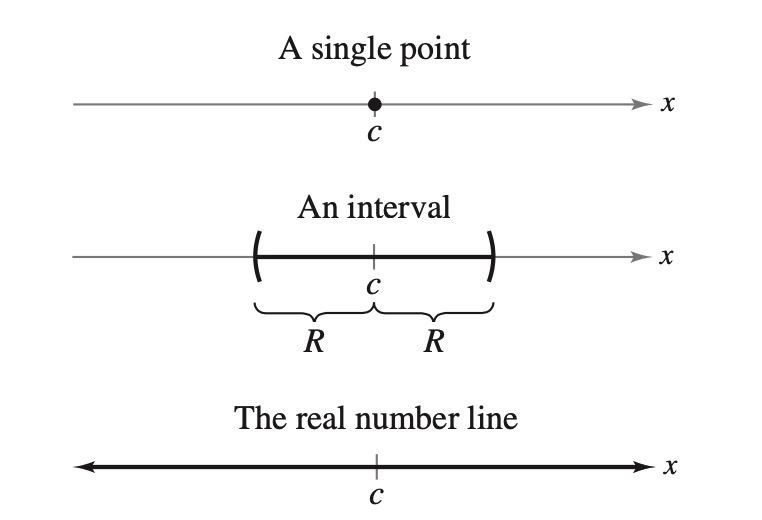
\includegraphics[width=0.50\linewidth]{Example_89.jpg} 
\end{minipage}


\begin{mytheorem}{Convergence of a Power Series}{}

For a power series centered at $c$, precisely one of the following is true:

\begin{enumerate}
    \item The series converges only at $c$.
    \item There exists a real number $R > 0$ such that the series converges absolutely for $\lvert x - c \rvert < R$ and diverges for $\lvert x - c \rvert > R$.
    \item The series converges absolutely for all $x$.
\end{enumerate}

The number $R$ is the \textbf{radius of convergence} of the power series. If the series converges only at $c$, then the radius of convergence is $R = 0$. If the series converges for all $x$, then the radius of convergence is $R = \infty$. The set of all values of $x$ for which the power series converges is the \textbf{interval of convergence} of the power series.
    
\end{mytheorem}


\begin{tcolorbox}[colback=examplebg, colframe=red!75!black, title=\textbf{EXAMPLE 2:Finding the Radius of Convergence}, fonttitle=\bfseries, sharp corners]

Find the radius of convergence of the power series $\sum_{n=0}^{\infty} n! x^n$.

\tcblower
\textbf{Solution:} 
For $x = 0$, you obtain
\[
f(0) = \sum_{n=0}^{\infty} n! \cdot 0^n = 1 + 0 + 0 + \cdots = 1.
\]
For any fixed value of $x$ such that $|x| > 0$, let $u_n = n! x^n$. Then,
\[
\lim_{n \to \infty} \left| \frac{u_{n+1}}{u_n} \right| = \lim_{n \to \infty} \left| \frac{(n+1)! x^{n+1}}{n! x^n} \right| = |x| \lim_{n \to \infty} (n+1) = \infty.
\]
Therefore, by the Ratio Test, the series diverges for $|x| > 0$ and converges only at its center, $0$. So, the radius of convergence is $R = 0$.
\end{tcolorbox}









\begin{tcolorbox}[colback=examplebg, colframe=red!75!black, title=\textbf{EXAMPLE 3: Finding the Radius of Convergence}, fonttitle=\bfseries, sharp corners]

Find the radius of convergence of the power series $\sum_{n=0}^{\infty} 3(x-2)^n$.

\tcblower
\textbf{Solution:} 
For $x \neq 2$, let $u_n = 3(x-2)^n$. Then,
\[
\lim_{n \to \infty} \left| \frac{u_{n+1}}{u_n} \right| = \lim_{n \to \infty} \left| \frac{3(x-2)^{n+1}}{3(x-2)^n} \right| = \lim_{n \to \infty} |x-2| = |x-2|.
\]
By the Ratio Test, the series converges for $|x-2| < 1$ and diverges for $|x-2| > 1$. Therefore, the radius of convergence of the series is $R = 1$.
\end{tcolorbox}





\begin{tcolorbox}[colback=examplebg, colframe=red!75!black, title=\textbf{EXAMPLE 4: Finding the Radius of Convergence}, fonttitle=\bfseries, sharp corners]

 Find the radius of convergence of the power series $\sum_{n=0}^{\infty} \frac{(-1)^n x^{2n+1}}{(2n+1)!}$.

\tcblower
\textbf{Solution:} 
Let $u_n = \frac{(-1)^n x^{2n+1}}{(2n+1)!}$. Then,
\[
\lim_{n \to \infty} \left| \frac{u_{n+1}}{u_n} \right| = \lim_{n \to \infty} \left| \frac{(-1)^{n+1} x^{2n+3}}{(2n+3)!} \cdot \frac{(2n+1)!}{(-1)^n x^{2n+1}} \right| = \lim_{n \to \infty} \frac{x^2}{(2n+3)(2n+2)}.
\]
For any fixed value of $x$, this limit is $0$. So, by the Ratio Test, the series converges for all $x$. Therefore, the radius of convergence is $R = \infty$.
\end{tcolorbox}

\newpage

\subsubsection{Endpoint Convergence}
\begin{Note}{Radius and Interval of Convergence}{}
    For a power series with a finite radius of convergence $R$, Theorem 9.20 does not specify the behavior at the \textbf{endpoints} of the interval of convergence. Each endpoint must be tested separately for convergence or divergence.

The interval of convergence can take one of six forms:
\begin{itemize}
    \item \textbf{Radius:} $0$ — The series converges only at the center $c$.
    \item \textbf{Radius:} $R$ — The interval may be:
    \begin{itemize}
        \item $(c-R, c+R)$
        \item $(c-R, c+R]$
        \item $[c-R, c+R)$
        \item $[c-R, c+R]$
    \end{itemize}
    \item \textbf{Radius:} $\infty$ — The series converges for all $x$.
\end{itemize}

\end{Note}

\begin{minipage}{\linewidth}
    \centering
    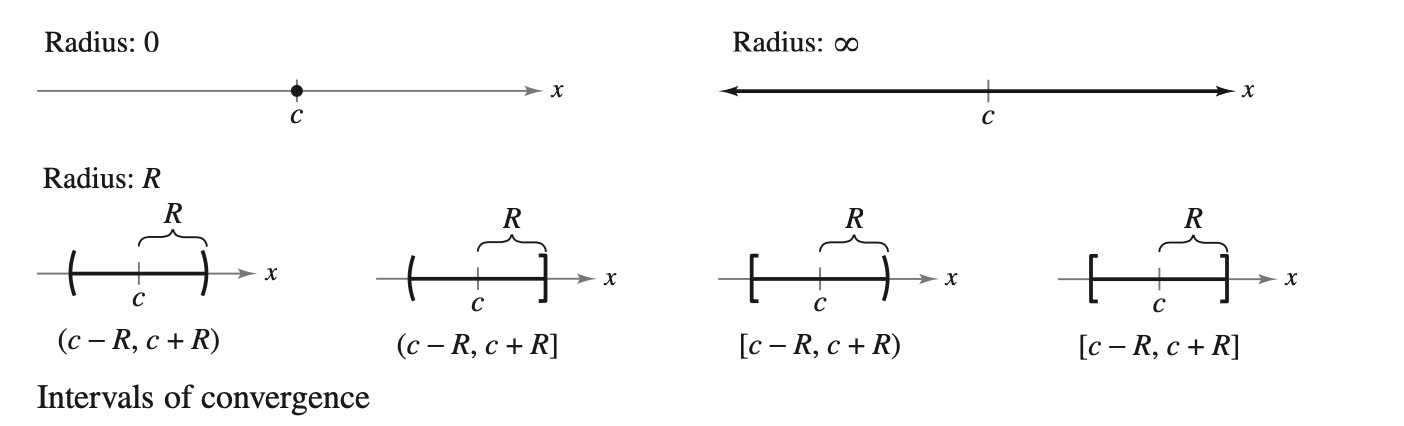
\includegraphics[width=1\linewidth]{Example_90.jpg} 
\end{minipage}

\newpage


\begin{tcolorbox}[colback=examplebg, colframe=red!75!black, title=\textbf{EXAMPLE 5: Finding the Interval of Convergence}, fonttitle=\bfseries, sharp corners]

Find the interval of convergence of 
\[
\sum_{n=1}^\infty \frac{x^n}{n}.
\]

\tcblower
\textbf{Solution:} 
Letting \( u_n = \frac{x^n}{n} \), we compute the ratio test:
\[
\lim_{n \to \infty} \left| \frac{u_{n+1}}{u_n} \right| = \lim_{n \to \infty} \left| \frac{x^{n+1}/(n+1)}{x^n/n} \right| = \lim_{n \to \infty} \left| \frac{nx}{n+1} \right| = |x|.
\]
So, by the Ratio Test, the radius of convergence is \( R = 1 \). The series converges in the interval \( (-1, 1) \), but we need to test convergence at each endpoint.

- For \( x = 1 \):
\[
\sum_{n=1}^\infty \frac{1}{n} \quad \text{(harmonic series, diverges).}
\]

- For \( x = -1 \):
\[
\sum_{n=1}^\infty \frac{(-1)^n}{n} \quad \text{(alternating harmonic series, converges).}
\]

Thus, the interval of convergence is \( [-1, 1) \).
\end{tcolorbox}




\begin{tcolorbox}[colback=examplebg, colframe=red!75!black, title=\textbf{EXAMPLE 6:  Finding the Interval of Convergence}, fonttitle=\bfseries, sharp corners]


Find the interval of convergence of 
\[
\sum_{n=0}^\infty \frac{(-1)^n (x+1)^n}{2^n}.
\]

\tcblower
\textbf{Solution:} 
Letting \( u_n = \frac{(-1)^n (x+1)^n}{2^n} \), we compute the ratio test:
\[
\lim_{n \to \infty} \left| \frac{u_{n+1}}{u_n} \right| = \lim_{n \to \infty} \left| \frac{(x+1)^{n+1}/2^{n+1}}{(x+1)^n/2^n} \right| = \lim_{n \to \infty} \left| \frac{x+1}{2} \right| = \frac{|x+1|}{2}.
\]
The series converges for 
\[
\frac{|x+1|}{2} < 1 \quad \Rightarrow \quad |x+1| < 2 \quad \Rightarrow \quad -3 < x < 1.
\]
At the endpoints:
- For \( x = -3 \): The series becomes 
\[
\sum_{n=0}^\infty \frac{(-1)^n (-2)^n}{2^n} = \sum_{n=0}^\infty (-1)^n = \text{(diverges).}
\]
- For \( x = 1 \): The series becomes 
\[
\sum_{n=0}^\infty \frac{(-1)^n (2)^n}{2^n} = \sum_{n=0}^\infty (-1)^n = \text{(diverges).}
\]

Thus, the interval of convergence is \( (-3, 1) \).
\end{tcolorbox}


\begin{tcolorbox}[colback=examplebg, colframe=red!75!black, title=\textbf{EXAMPLE 7: Finding the Interval of Convergence}, fonttitle=\bfseries, sharp corners]
Find the interval of convergence of 
\[
\sum_{n=1}^\infty \frac{x^n}{n^2}.
\]


\tcblower
\textbf{Solution:} 
Letting \( u_n = \frac{x^n}{n^2} \), we compute the ratio test:
\[
\lim_{n \to \infty} \left| \frac{u_{n+1}}{u_n} \right| = \lim_{n \to \infty} \left| \frac{x^{n+1}/(n+1)^2}{x^n/n^2} \right| = \lim_{n \to \infty} \left| \frac{n^2 x}{(n+1)^2} \right| = |x|.
\]
So, by the Ratio Test, the radius of convergence is \( R = 1 \). The series converges in the interval \( (-1, 1) \), but we need to test convergence at each endpoint.

- For \( x = 1 \):
\[
\sum_{n=1}^\infty \frac{1}{n^2} \quad \text{(p-series, converges for \( p > 1 \)).}
\]

- For \( x = -1 \):
\[
\sum_{n=1}^\infty \frac{(-1)^n}{n^2} \quad \text{(alternating series, converges).}
\]

Thus, the interval of convergence is \( [-1, 1] \).
\end{tcolorbox}


\subsubsection{Differentiation and Integration of Power Series}

\begin{mytheorem}{Properties of Functions Defined by Power Series}{}

If the function 
\[
f(x) = \sum_{n=0}^\infty a_n (x-c)^n = a_0 + a_1(x-c) + a_2(x-c)^2 + a_3(x-c)^3 + \cdots
\]
has a radius of convergence of $R > 0$, then, on the interval $(c-R, c+R)$, $f$ is differentiable (and therefore continuous). Moreover, the derivative and antiderivative of $f$ are as follows:

1. Derivative:
\[
f'(x) = \sum_{n=1}^\infty n a_n (x-c)^{n-1} = a_1 + 2a_2(x-c) + 3a_3(x-c)^2 + \cdots
\]

2. Antiderivative:
\[
\int f(x) dx = C + \sum_{n=0}^\infty \frac{a_n (x-c)^{n+1}}{n+1} = C + a_0(x-c) + \frac{a_1(x-c)^2}{2} + \frac{a_2(x-c)^3}{3} + \cdots
\]

The \textit{radius of convergence} of the series obtained by differentiating or integrating a power series is the same as that of the original power series. The \textit{interval of convergence}, however, may differ as a result of the behavior at the endpoints.
    
\end{mytheorem}



\begin{tcolorbox}[colback=examplebg, colframe=red!75!black, title=\textbf{EXAMPLE 8: Intervals of Convergence for $f(x)$, $f'(x)$, and $\int f(x) dx$}, fonttitle=\bfseries, sharp corners]

Consider the function 
\[
f(x) = \sum_{n=1}^\infty \frac{x^n}{n} = x + \frac{x^2}{2} + \frac{x^3}{3} + \cdots
\]

Find the interval of convergence for each of the following:
\begin{enumerate}[a.]
    \item $\int f(x) dx$
    \item $f(x)$
    \item $f'(x)$
\end{enumerate}

\tcblower
\textbf{Solution:} 
 By Theorem, we have:
\[
f'(x) = \sum_{n=1}^\infty x^{n-1} = 1 + x + x^2 + \cdots
\]
and
\[
\int f(x) dx = C + \sum_{n=1}^\infty \frac{x^{n+1}}{n(n+1)} = C + x + \frac{x^2}{2 \cdot 2} + \frac{x^3}{3 \cdot 3} + \cdots
\]

Using the Ratio Test, each series has a radius of convergence of $R = 1$. Considering the interval $(-1, 1)$, we determine:

\begin{enumerate}[a.]
    \item For $\int f(x) dx$, the series 
    \[
    \sum_{n=1}^\infty \frac{x^{n+1}}{n(n+1)}
    \]
    converges for $x = \pm 1$. Thus, the interval of convergence is $[-1, 1]$.

    \item For $f(x)$, the series 
    \[
    \sum_{n=1}^\infty \frac{x^n}{n}
    \]
    converges for $x = -1$ and diverges for $x = 1$. Thus, the interval of convergence is $[-1, 1)$.

    \item For $f'(x)$, the series 
    \[
    \sum_{n=1}^\infty x^{n-1}
    \]
    diverges for $x = \pm 1$. Thus, the interval of convergence is $(-1, 1)$.
\end{enumerate}
\end{tcolorbox}

\subsection{Taylor or Maclaurin Series for a Function}
\subsubsection{Taylor Series and Maclaurin Series}
In the previous chapter, you derived power series for several functions using geometric series with term-by-term differentiation or integration. In this section, you will study a general procedure for deriving the power series for a function that has derivatives of all orders.


\begin{mytheorem}{The Form of a Convergent Power Series}{}
    If a function $f$ is represented by a power series 
\[
f(x) = \sum_{n=0}^\infty a_n (x-c)^n
\]
for all $x$ in an open interval $I$ containing $c$, then 
\[
a_n = \frac{f^{(n)}(c)}{n!}.
\]

Thus, 
\[
f(x) = f(c) + f'(c)(x-c) + \frac{f''(c)}{2!}(x-c)^2 + \dots + \frac{f^{(n)}(c)}{n!}(x-c)^n + \dots.
\]

\end{mytheorem}


\begin{Definition}{Taylor and Maclaurin Series}{}

If a function $f$ has derivatives of all orders at $x=c$, then the series 
\[
\sum_{n=0}^\infty \frac{f^{(n)}(c)}{n!}(x-c)^n = f(c) + f'(c)(x-c) + \dots + \frac{f^{(n)}(c)}{n!}(x-c)^n + \dots
\]
is called the \textbf{Taylor series} for $f(x)$ at $c$. Moreover, if $c=0$, then the series is the \textbf{Maclaurin series} for $f$.
\end{Definition}

\begin{tcolorbox}[colback=examplebg, colframe=red!75!black, title=\textbf{EXAMPLE 1: Forming a Power Series}, fonttitle=\bfseries, sharp corners]

Use the function 
\[
f(x) = \sin x
\]
to form the Maclaurin series 
\[
\sum_{n=0}^\infty \frac{f^{(n)}(0)}{n!}x^n = f(0) + f'(0)x + \frac{f''(0)}{2!}x^2 + \frac{f^{(3)}(0)}{3!}x^3 + \frac{f^{(4)}(0)}{4!}x^4 + \dots
\]
and determine the interval of convergence.

\tcblower
\textbf{Solution:} 
Successive differentiation of $f(x)$ yields:
\[
f(x) = \sin x, \quad f'(x) = \cos x, \quad f''(x) = -\sin x, \quad f^{(3)}(x) = -\cos x,
\]
\[
f^{(4)}(x) = \sin x, \quad f^{(5)}(x) = \cos x, \quad \dots
\]
Evaluating these derivatives at $x = 0$, we have:
\[
f(0) = \sin 0 = 0, \quad f'(0) = \cos 0 = 1, \quad f''(0) = -\sin 0 = 0, \quad f^{(3)}(0) = -\cos 0 = -1,
\]
\[
f^{(4)}(0) = \sin 0 = 0, \quad f^{(5)}(0) = \cos 0 = 1, \quad \dots
\]
The pattern repeats after the third derivative.

The Maclaurin series is:
\[
\sum_{n=0}^\infty \frac{f^{(n)}(0)}{n!}x^n = f(0) + f'(0)x + \frac{f''(0)}{2!}x^2 + \frac{f^{(3)}(0)}{3!}x^3 + \dots
\]
Substituting the values of the derivatives:
\[
\sum_{n=0}^\infty \frac{(-1)^n x^{2n+1}}{(2n+1)!} = 0 + (1)x + \frac{0}{2!}x^2 + \frac{-1}{3!}x^3 + \frac{0}{4!}x^4 + \frac{1}{5!}x^5 + \frac{0}{6!}x^6 + \frac{-1}{7!}x^7 + \dots
\]
Simplifying, we get:
\[
\sin x = x - \frac{x^3}{3!} + \frac{x^5}{5!} - \frac{x^7}{7!} + \dots
\]

Also, by using ratio test, we could conclude that the series is convergent to $f(x)$
\end{tcolorbox}

\begin{mytheorem}{ Convergence of Taylor Series}{}
    If 
\[
\lim_{n \to \infty} R_n = 0
\]
for all $x$ in the interval $I$, then the Taylor series for $f$ converges and equals $f(x)$:
\[
f(x) = \sum_{n=0}^\infty \frac{f^{(n)}(c)}{n!}(x - c)^n.
\]
\end{mytheorem}


\begin{Note}{Guidelines for Finding a Taylor Series}{}
    \begin{enumerate}
    \item Differentiate $f(x)$ several times and evaluate each derivative at $c$.
    \[
    f(c), \, f'(c), \, f''(c), \, f'''(c), \, \dots, \, f^{(n)}(c), \, \dots
    \]
    Try to recognize a pattern in these numbers.
    \item Use the sequence developed in the first step to form the Taylor coefficients 
    \[
    a_n = \frac{f^{(n)}(c)}{n!},
    \]
    and determine the interval of convergence for the resulting power series:
    \[
    f(c) + f'(c)(x - c) + \frac{f''(c)}{2!}(x - c)^2 + \dots + \frac{f^{(n)}(c)}{n!}(x - c)^n + \dots
    \]
    \item Within this interval of convergence, determine whether the series converges to $f(x)$.
\end{enumerate}
\end{Note}


\begin{tcolorbox}[colback=examplebg, colframe=red!75!black, title=\textbf{EXAMPLE 2: Maclaurin Series for a Composite Function}, fonttitle=\bfseries, sharp corners]
Find the Maclaurin series for $f(x) = \sin x^2$.


\tcblower
\textbf{Solution:} 
To find the coefficients for this Maclaurin series directly, you must calculate successive derivatives of $f(x) = \sin x^2$. By calculating just the first two,
\[
f'(x) = 2x \cos x^2
\]
and
\[
f''(x) = -4x^2 \sin x^2 + 2 \cos x^2.
\]
You can see that this task would be quite cumbersome. Fortunately, there is an alternative. First, consider the Maclaurin series for $\sin x$ found in Example 1.

Let $g(x) = \sin x$, so
\[
g(x) = x - \frac{x^3}{3!} + \frac{x^5}{5!} - \frac{x^7}{7!} + \dots
\]
Now, because $\sin x^2 = g(x^2)$, you can substitute $x^2$ for $x$ in the series for $\sin x$ to obtain
\[
\sin x^2 = g(x^2) = x^2 - \frac{x^6}{3!} + \frac{x^{10}}{5!} - \frac{x^{14}}{7!} + \dots
\]
\end{tcolorbox}

\newpage
\subsubsection{Binomial Series}

\begin{mytheorem}{Binomial Theorem}{}

If $n$ is any positive integer, then
\[
(a + b)^n = \sum_{i=0}^n \binom{n}{i} a^{n-i}b^i = a^n + na^{n-1}b + \frac{n(n-1)}{2!}a^{n-2}b^2 + \cdots + nab^{n-1} + b^n,
\]
where
\[
\binom{n}{i} = \frac{n(n-1)(n-2)\cdots(n-i+1)}{i!}, \quad i = 1, 2, 3, \dots, n,
\]
and
\[
\binom{n}{0} = 1.
\]
    
\end{mytheorem}

\begin{mytheorem}{Binomial Series}{}
   If $k$ is any number and $\lvert x \rvert < 1$, then
\[
(1 + x)^k = \sum_{n=0}^\infty \binom{k}{n}x^n = 1 + kx + \frac{k(k-1)}{2!}x^2 + \frac{k(k-1)(k-2)}{3!}x^3 + \cdots.
\] 
\end{mytheorem}


\begin{tcolorbox}[colback=examplebg, colframe=red!75!black, title=\textbf{EXAMPLE 3: Binomial Series}, fonttitle=\bfseries, sharp corners]

Find the Maclaurin series for $f(x) = (1+x)^k$ and determine its radius of convergence. Assume that $k$ is not a positive integer and $k \neq 0$.


\tcblower
\textbf{Solution:} 
By successive differentiation, you have:
\[
f(x) = (1+x)^k \quad \Rightarrow \quad f'(x) = k(1+x)^{k-1}, \quad f''(x) = k(k-1)(1+x)^{k-2},
\]
\[
f^{(3)}(x) = k(k-1)(k-2)(1+x)^{k-3}, \quad \dots \quad f^{(n)}(x) = k(k-1)\dots(k-n+1)(1+x)^{k-n}.
\]
At $x = 0$, this produces:
\[
f(0) = 1, \quad f'(0) = k, \quad f''(0) = k(k-1), \quad f^{(3)}(0) = k(k-1)(k-2), \quad \dots
\]
The series is:
\[
1 + kx + \frac{k(k-1)x^2}{2} + \frac{k(k-1)(k-2)x^3}{3!} + \dots + \frac{k(k-1)\dots(k-n+1)x^n}{n!} + \dots
\]
By the Ratio Test, the radius of convergence is $R=1$, so the series converges for $x \in (-1,1)$.
\end{tcolorbox}



\begin{tcolorbox}[colback=examplebg, colframe=red!75!black, title=\textbf{EXAMPLE 4: Finding a Binomial Series}, fonttitle=\bfseries, sharp corners]

Find the power series for $f(x) = \sqrt[3]{1+x}$.

\tcblower
\textbf{Solution:} 
Using the binomial series:
\[
(1+x)^k = 1 + kx + \frac{k(k-1)x^2}{2!} + \frac{k(k-1)(k-2)x^3}{3!} + \dots,
\]
let $k = \frac{1}{3}$ and write:
\[
(1+x)^{1/3} = 1 + \frac{x}{3} - \frac{2x^2}{3 \cdot 2!} + \frac{2 \cdot 5x^3}{3^3 \cdot 3!} - \frac{2 \cdot 5 \cdot 8x^4}{3^4 \cdot 4!} + \dots
\]
This series converges for $-1 \leq x \leq 1$.
\end{tcolorbox}
\newpage


\subsubsection{POWER SERIES FOR ELEMENTARY FUNCTIONS}

\begin{tcolorbox}[colframe=blue!75!black, colback=white, title=Power Series Representations, sharp corners]
\[
\frac{1}{1-x} = \sum_{n=0}^\infty x^n = 1 + x + x^2 + x^3 + \cdots, \quad R = 1
\]

\[
e^x = \sum_{n=0}^\infty \frac{x^n}{n!} = 1 + \frac{x}{1!} + \frac{x^2}{2!} + \frac{x^3}{3!} + \cdots, \quad R = \infty
\]

\[
\sin x = \sum_{n=0}^\infty \frac{(-1)^n x^{2n+1}}{(2n+1)!} = x - \frac{x^3}{3!} + \frac{x^5}{5!} - \frac{x^7}{7!} + \cdots, \quad R = \infty
\]

\[
\cos x = \sum_{n=0}^\infty \frac{(-1)^n x^{2n}}{(2n)!} = 1 - \frac{x^2}{2!} + \frac{x^4}{4!} - \frac{x^6}{6!} + \cdots, \quad R = \infty
\]

\[
\arctan x = \sum_{n=0}^\infty \frac{(-1)^n x^{2n+1}}{2n+1} = x - \frac{x^3}{3} + \frac{x^5}{5} - \frac{x^7}{7} + \cdots, \quad R = 1
\]

\[
\ln(1+x) = \sum_{n=1}^\infty \frac{(-1)^{n-1} x^n}{n} = x - \frac{x^2}{2} + \frac{x^3}{3} - \frac{x^4}{4} + \cdots, \quad R = 1
\]

\[
(1+x)^k = \sum_{n=0}^\infty \binom{k}{n} x^n = 1 + kx + \frac{k(k-1)}{2!}x^2 + \frac{k(k-1)(k-2)}{3!}x^3 + \cdots, \quad R = 1
\]
\end{tcolorbox}



\begin{tcolorbox}[colback=examplebg, colframe=red!75!black, title=\textbf{EXAMPLE 5: Deriving a Power Series from a Basic List}, fonttitle=\bfseries, sharp corners]

Find the power series for 
\[
f(x) = \cos \sqrt{x}.
\]

\tcblower
\textbf{Solution:} 
Using the power series for $\cos x$, we have:
\[
\cos x = 1 - \frac{x^2}{2!} + \frac{x^4}{4!} - \frac{x^6}{6!} + \frac{x^8}{8!} - \cdots
\]

Replace $x$ by $\sqrt{x}$:
\[
\cos \sqrt{x} = 1 - \frac{x}{2!} + \frac{x^2}{4!} - \frac{x^3}{6!} + \frac{x^4}{8!} - \cdots
\]

This series converges for all $x \geq 0$.
\end{tcolorbox}



\begin{tcolorbox}[colback=examplebg, colframe=red!75!black, title=\textbf{EXAMPLE 6: Multiplication of Power Series}, fonttitle=\bfseries, sharp corners]

Find the first three nonzero terms in the Maclaurin series for $e^x \arctan x$.

\tcblower
\textbf{Solution:} 
Using the Maclaurin series for $e^x$ and $\arctan x$:
\[
e^x = 1 + \frac{x}{1!} + \frac{x^2}{2!} + \frac{x^3}{3!} + \frac{x^4}{4!} + \cdots
\]
\[
\arctan x = x - \frac{x^3}{3} + \frac{x^5}{5} - \cdots
\]

Multiply these expressions:
\[
e^x \arctan x = \left( 1 + \frac{x}{1!} + \frac{x^2}{2!} + \frac{x^3}{3!} + \frac{x^4}{4!} + \cdots \right) 
\left( x - \frac{x^3}{3} + \frac{x^5}{5} - \cdots \right).
\]

Expand and collect like terms:
\[
e^x \arctan x = x + x^2 + \frac{x^3}{6} - \frac{x^3}{3} + \cdots
\]
\[
e^x \arctan x = x + x^2 - \frac{x^3}{6} + \frac{x^5}{40} + \cdots
\]

So, the first three nonzero terms are:
\[
e^x \arctan x = x + x^2 + \frac{x^3}{6} + \cdots
\]
\end{tcolorbox}


\begin{tcolorbox}[colback=examplebg, colframe=red!75!black, title=\textbf{EXAMPLE 7:  Maclaurin Series}, fonttitle=\bfseries, sharp corners]
Find the Maclaurin series for:

\begin{itemize}
    \item[(a)] $f(x) = x \cos x$
    \item[(b)] $f(x) = \ln(1 + 3x^2)$
\end{itemize}


\tcblower
\textbf{Solution:} 
\noindent \textbf{(a)} Using the Maclaurin series for $\cos x$, we multiply by $x$:
\[
\cos x = \sum_{n=0}^\infty \frac{(-1)^n x^{2n}}{(2n)!}
\]
\[
x \cos x = x \sum_{n=0}^\infty \frac{(-1)^n x^{2n}}{(2n)!} = \sum_{n=0}^\infty \frac{(-1)^n x^{2n+1}}{(2n)!}, \quad \text{for all } x.
\]

\noindent \textbf{(b)} Replacing $x$ by $3x^2$ in the Maclaurin series for $\ln(1+x)$:
\[
\ln(1+x) = \sum_{n=1}^\infty \frac{(-1)^{n-1} x^n}{n}
\]
\[
\ln(1+3x^2) = \sum_{n=1}^\infty \frac{(-1)^{n-1} (3x^2)^n}{n} = \sum_{n=1}^\infty \frac{(-1)^{n-1} 3^n x^{2n}}{n}.
\]

\noindent, this series converges for $\lvert 3x^2 \rvert < 1$, that is, $\lvert x \rvert < \frac{1}{\sqrt{3}}$, so the radius of convergence is:
\[
R = \frac{1}{\sqrt{3}}.
\]
\end{tcolorbox}



\begin{tcolorbox}[colback=examplebg, colframe=red!75!black, title=\textbf{EXAMPLE 8: Power Series Approximation of a Definite Integral}, fonttitle=\bfseries, sharp corners]

Use a power series to approximate:
\[
\int_0^1 e^{-x^2} \, dx
\]
with an error of less than $0.01$.

\tcblower
\textbf{Solution:} 
Using the power series for $e^x$:
\[
e^x = 1 + x + \frac{x^2}{2!} + \frac{x^3}{3!} + \cdots,
\]
replace $x$ with $-x^2$:
\[
e^{-x^2} = 1 - x^2 + \frac{x^4}{2!} - \frac{x^6}{3!} + \cdots.
\]

Now, integrate term by term:
\[
\int_0^1 e^{-x^2} \, dx = \int_0^1 \left( 1 - x^2 + \frac{x^4}{2!} - \frac{x^6}{3!} + \cdots \right) dx.
\]

Integrate each term:
\[
\int_0^1 e^{-x^2} \, dx = \left[ x - \frac{x^3}{3} + \frac{x^5}{5 \cdot 2!} - \frac{x^7}{7 \cdot 3!} + \cdots \right]_0^1.
\]

Substitute the limits:
\[
\int_0^1 e^{-x^2} \, dx = 1 - \frac{1}{3} + \frac{1}{10} - \frac{1}{42} + \cdots.
\]

Summing the first four terms:
\[
\int_0^1 e^{-x^2} \, dx \approx 0.74,
\]
which has an error less than $0.01$.
\end{tcolorbox}
\newpage
\subsection{Representing
Functions as
Power Series}

In the previous chapter, If $x$ is a variable, then an infinite series of the form

\[
\sum_{n=0}^\infty a_n x^n = a_0 + a_1 x + a_2 x^2 + a_3 x^3 + \cdots + a_n x^n + \cdots
\]

is called a \textit{power series}. 

In this section, we will study several techniques for finding a power series that represents a function. Consider the function.

\subsubsection{Geometric Power Series}

\begin{Note}{Geometric Power Series}{}

Consider the function:
\[
f(x) = \frac{1}{1-x}.
\]

This function resembles the sum of a geometric series:
\[
\sum_{n=0}^\infty ar^n = \frac{a}{1-r}, \quad \text{for } 0 < |r| < 1.
\]

When $a = 1$ and $r = x$, the power series representation for $\frac{1}{1-x}$, centered at $0$, is:
\[
\frac{1}{1-x} = \sum_{n=0}^\infty x^n = 1 + x + x^2 + x^3 + \cdots, \quad \text{for } |x| < 1.
\]
    
\end{Note}

\begin{tcolorbox}[colback=examplebg, colframe=red!75!black, title=\textbf{EXAMPLE 1: Finding a Geometric Power Series Centered at 0}, fonttitle=\bfseries, sharp corners]

Find a power series for $f(x) = \frac{4}{x+2}$ centered at $0$.

\tcblower
\textbf{Solution:} 
Writing $f(x)$ in the form $\frac{a}{1-r}$ produces:
\[
\frac{4}{x+2} = \frac{2}{1 - \left(-\frac{x}{2}\right)} = \frac{a}{1-r},
\]
which implies that $a = 2$ and $r = -\frac{x}{2}$.

So, the power series for $f(x)$ is:
\[
\frac{4}{x+2} = \sum_{n=0}^\infty ar^n = \sum_{n=0}^\infty 2\left(-\frac{x}{2}\right)^n = 2\left(1 - \frac{x}{2} + \frac{x^2}{4} - \frac{x^3}{8} + \cdots \right).
\]

This power series converges when:
\[
\left| -\frac{x}{2} \right| < 1,
\]
which implies that the interval of convergence is $(-2, 2)$.
\end{tcolorbox}

\newpage
\subsubsection{Operations with Power Series}
\begin{Note}{Operations with Power Series}{}
Let 
\[
f(x) = \sum_{n=0}^\infty a_n x^n \quad \text{and} \quad g(x) = \sum_{n=0}^\infty b_n x^n.
\]

\begin{enumerate}
    \item $f(kx) = \sum_{n=0}^\infty a_n k^n x^n$
    \item $f(x^N) = \sum_{n=0}^\infty a_n x^{nN}$
    \item $f(x) \pm g(x) = \sum_{n=0}^\infty (a_n \pm b_n)x^n$
\end{enumerate}
\end{Note}
\begin{tcolorbox}[colback=examplebg, colframe=red!75!black, title=\textbf{EXAMPLE 2: Adding Two Power Series}, fonttitle=\bfseries, sharp corners]
Find a power series for 
\[
f(x) = \frac{3x - 1}{x^2 - 1}
\]
centered at $0$.



\tcblower
\textbf{Solution:} 
Using partial fractions, we rewrite $f(x)$:
\[
\frac{3x - 1}{x^2 - 1} = \frac{2}{x + 1} + \frac{1}{x - 1}.
\]

Each term can be expressed as a geometric power series:
\[
\frac{2}{x + 1} = 2 \cdot \frac{1}{1 - (-x)} = \sum_{n=0}^\infty 2(-1)^n x^n, \quad |x| < 1,
\]
\[
\frac{1}{x - 1} = -\frac{1}{1 - x} = -\sum_{n=0}^\infty x^n, \quad |x| < 1.
\]

Adding these two series, we obtain:
\[
\frac{3x - 1}{x^2 - 1} = \sum_{n=0}^\infty [2(-1)^n - 1]x^n = 1 - 3x + x^2 - 3x^3 + x^4 - \cdots.
\]

The interval of convergence for this series is $(-1, 1)$.
\end{tcolorbox}

\begin{tcolorbox}[colback=examplebg, colframe=red!75!black, title=\textbf{EXAMPLE 3: Finding a Power Series by Integration}, fonttitle=\bfseries, sharp corners]

Find a power series for 
\[
f(x) = \ln x
\]
centered at $1$.

\tcblower
\textbf{Solution:} 
\[
\frac{1}{x} = \sum_{n=0}^\infty (-1)^n(x - 1)^n, \quad |x - 1| < 1.
\]

Integrating this series:
\[
\ln x = \int \frac{1}{x} \, dx + C = \sum_{n=0}^\infty \frac{(-1)^n (x - 1)^{n+1}}{n + 1} + C.
\]

By letting $x = 1$, we find $C = 0$, so:
\[
\ln x = \sum_{n=0}^\infty \frac{(-1)^n (x - 1)^{n+1}}{n + 1} = (x - 1) - \frac{(x - 1)^2}{2} + \frac{(x - 1)^3}{3} - \frac{(x - 1)^4}{4} + \cdots.
\]

The interval of convergence is $(0, 2)$.
\end{tcolorbox}


\begin{tcolorbox}[colback=examplebg, colframe=red!75!black, title=\textbf{EXAMPLE 4: Finding a Power Series by Integration}, fonttitle=\bfseries, sharp corners]

Find a power series for 
\[
g(x) = \arctan x
\]
centered at $0$.


\tcblower
\textbf{Solution:} 
Since $\frac{d}{dx}[\arctan x] = \frac{1}{1 + x^2}$, we use the series for $\frac{1}{1 + x^2}$:
\[
\frac{1}{1 + x^2} = \sum_{n=0}^\infty (-1)^n x^{2n}.
\]

Integrating term by term:
\[
\arctan x = \int \frac{1}{1 + x^2} \, dx + C = \sum_{n=0}^\infty \frac{(-1)^n x^{2n+1}}{2n + 1} + C.
\]

Letting $x = 0$ gives $C = 0$, so:
\[
\arctan x = \sum_{n=0}^\infty \frac{(-1)^n x^{2n+1}}{2n + 1} = x - \frac{x^3}{3} + \frac{x^5}{5} - \frac{x^7}{7} + \cdots.
\]

The interval of convergence is $(-1, 1)$.
\end{tcolorbox}
\end{document}
